%%____________________________________________________________________________||
\section{Results}
\label{sec:results}

The following section summarises the result of this analysis. The
control regions are populated with the full data set of 2016, namely
35.9\fbinv. As indicated in Sec.~\ref{sec:blinding}, the signal region
has been fully unblinded. 

Two different fits are performed. The {\it control-region-only fit} or
{\it masked fit} is constrained by data in the control regions only
and does not consider the observed data counts in the signal
region. The {\it signal-region fit} or {\it full fit} is constrained
by data counts in all control and signal regions, under the assumption that no
signal is present. 
(Note that the terms
{\it masked fit} and {\it control-region-only fit} ({\it CR-only fit})
are also used interchangeably.)

Figures~\ref{fig:cr-fit} and \ref{fig:full-fit} show the results of the control region-only fit and full fit respectively, for the signal region bins (\nj, \nb, \scalht, and \mht).
For each fit, the results are divided into six figures containing the seven considered event topologies, with monojet and asymmetric events shown together.

Each of these figures contains three panels.  The top panels show the
event yields in the signal region as observed in data (solid circles) and as
predicted in the SM (black histogram).  The uncertainties on the prediction are
indicated by the shaded bands, with the grey band for the uncertainty on the
total prediction and the burgundy shaded band for the remnant multi-jet
background.

Central panels show the ratio of the observed and expected counts.
Error bars contain both statistical and systematic uncertainties and show the
mid-P interval for the ratio.

Finally, the bottom panels provide the observed pull of the data given by the
difference between observed and expected yields and normalised to the total
uncertainty.  The total uncertainty is the quadrature sum of the uncertainty on
the prediction and the asymmetric statistical uncertainty on the data. The
upper (lower) value of the statistical uncertainty on the data is used when the
prediction is above (below) the observed value.

%Figures~\ref{fig:mr_mono_pre} and \ref{fig:mr_mono_post} summarise the
%event yields observed in data and SM expectations with their
%associated uncertainties as a function of \scalht and \nb, integated
%over \mht, for the monojet category ($\njet = 1$) for the masked and
%full fits, respectively. The lower panels show the data-to-background
%ratios for the masked and full fits.  Figure~\ref{fig:mr_mono_pulls}
%shows background expectations for the masked fit in the upper panel,
%as shown in Fig.~\ref{fig:mr_mono_pre}, and the pulls (\ie the
%difference between data and the background estimates relative to their
%uncertainties) for both the masked and full fits in the lower
%panel. 
%The same information is shown in Figs.~\ref{fig:mr_asym_pre},
%\ref{fig:mr_asym_post}, \ref{fig:mr_asym_pulls} and
%\ref{fig:mr_symm_pre}, \ref{fig:mr_symm_post}, \ref{fig:mr_symm_pulls}
%for the asymmetric and symmetric \njet categories,
%respectively. 

Figure~\ref{fig:ratios_and_pulls} shows histograms of the masked fit
values of the data-to-background ratios and pulls for all event
categories. Figure~\ref{fig:pulls} shows the pulls as a function of
(\njet, \nb) event category and \scalht, with counts integrated over
\mht, obtained from the masked fit.
%A goodness-of-fit estimate can be obtained by considering the pulls
%obtained from the masked fit, which in the following are assumed to be
%derived from independent background estimates. The summation over the
%squares of the pulls from 101 (\njet, \nb, \scalht) categories,
%summarised in Fig.~\ref{fig:pulls}, gives a $\chi^2$ value of
%73.0. Hence the reduced $\chi^2$ and the p-value are 0.72 and 0.98,
%respectively.

Figure~\ref{fig:breakdown} provides the breakdown of SM backgrounds
(categorised as lost lepton, \znunuj, or multijet) in the signal
region as determined from the CR-only and full fits.

%Appendix~\ref{app:mhtshapes} contains figures that show the event
%yields observed in data and CR-fit SM expectations with their
%associated uncertainties as a function of \HTmiss for each (\njet,
%\nb) event category and \scalht bin.
Additional figures can be found in the appendix.
Appendix~\ref{app:nuispost}
contains figures showing the post-fit behaviour of the nuisance
parameters relative to their pre-fit values.
The results with the simplified binning scheme, described in
Sec.~\ref{sec:aggregated}, are shown in Appendix~\ref{app:aggregated} in
figures~\ref{fig:aggregated_results1},
\ref{fig:aggregated_results2}, \ref{fig:aggregated_results3}, and
\ref{fig:aggregated_results4}.

\clearpage
\begin{figure}[!h]
  \centering
  \subfigure[\label{fig:cr-fit:mono-asymm}Monojet and asymmetric topologies]{
    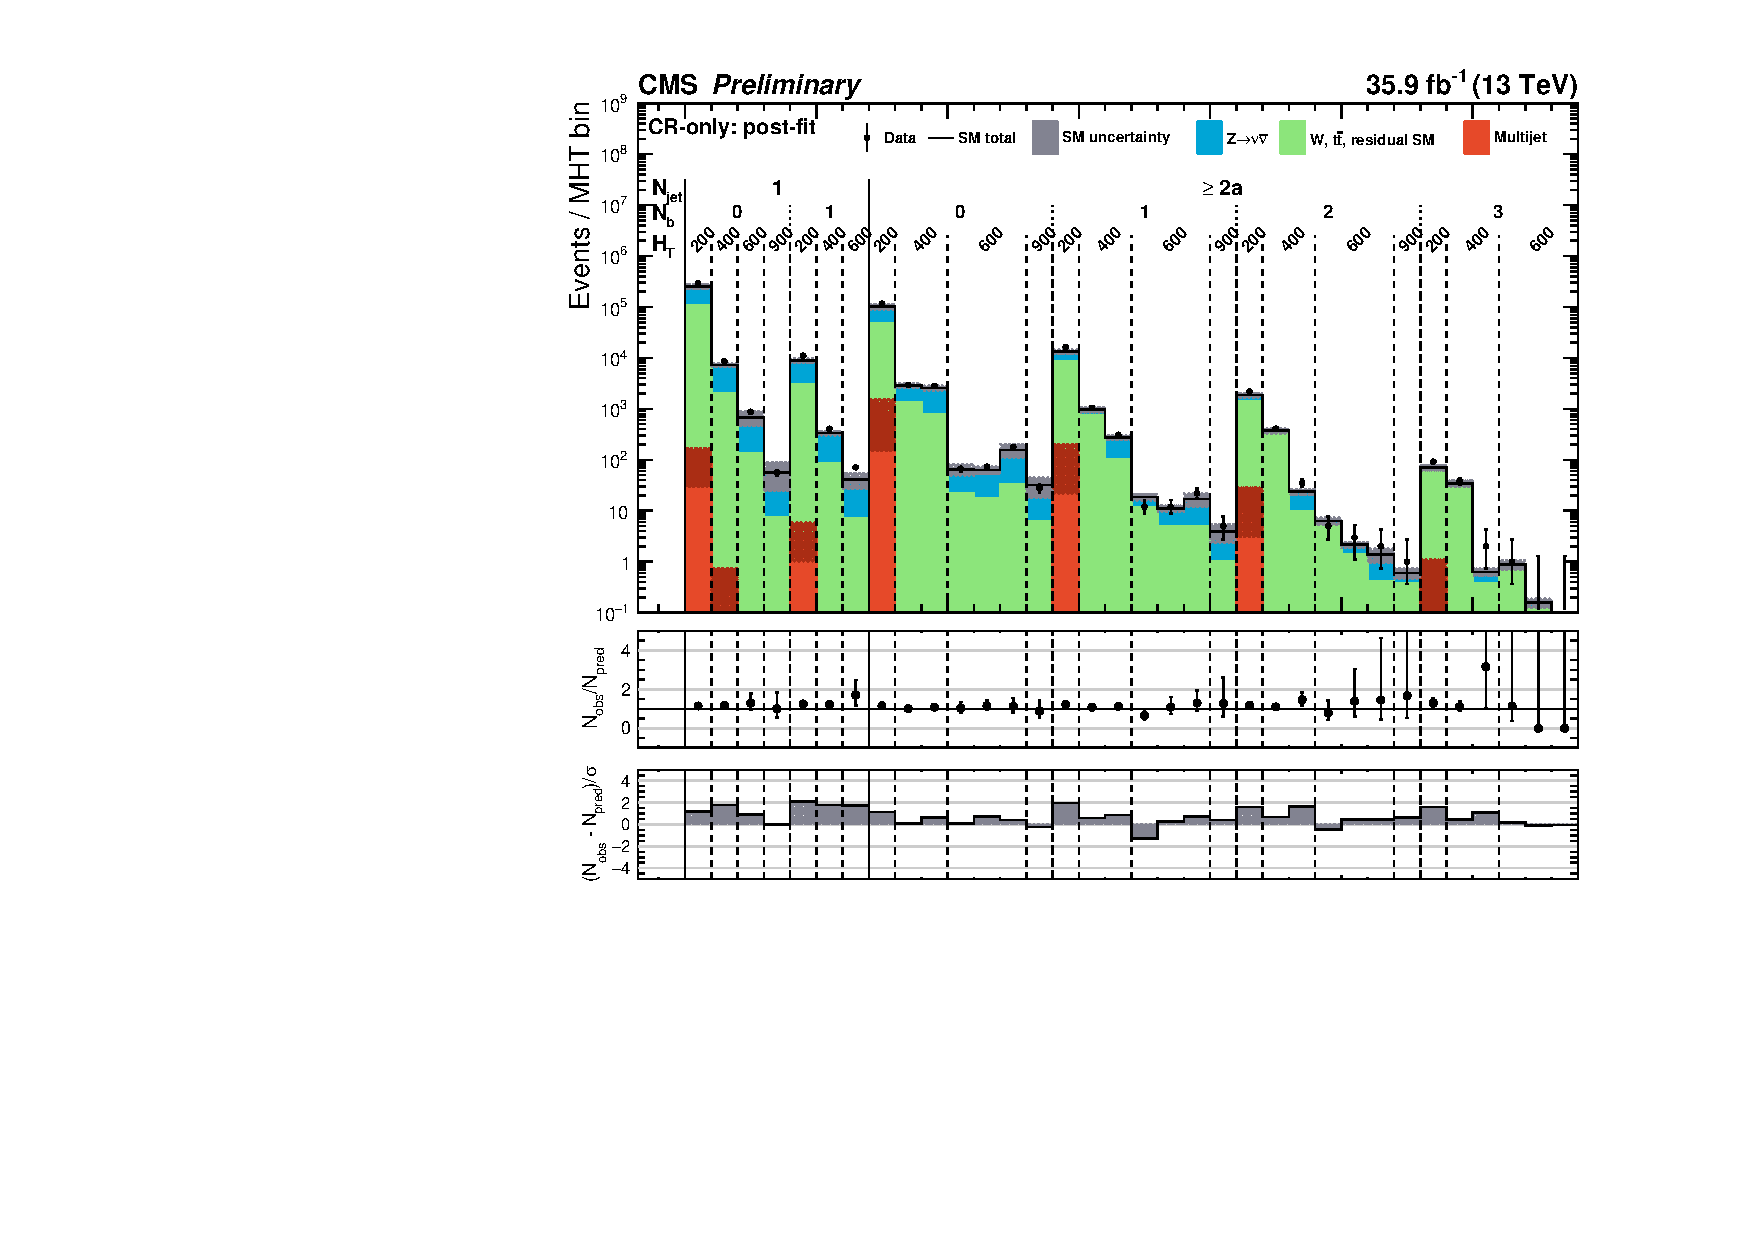
\includegraphics[width=0.48\textwidth]{figures/results/36invfb_preapproval/mht_binned/prefit/monojet_prefit_dists_true.pdf}
  }~ 
  \subfigure[\label{fig:cr-fit:dijet}Dijet topologies]{
    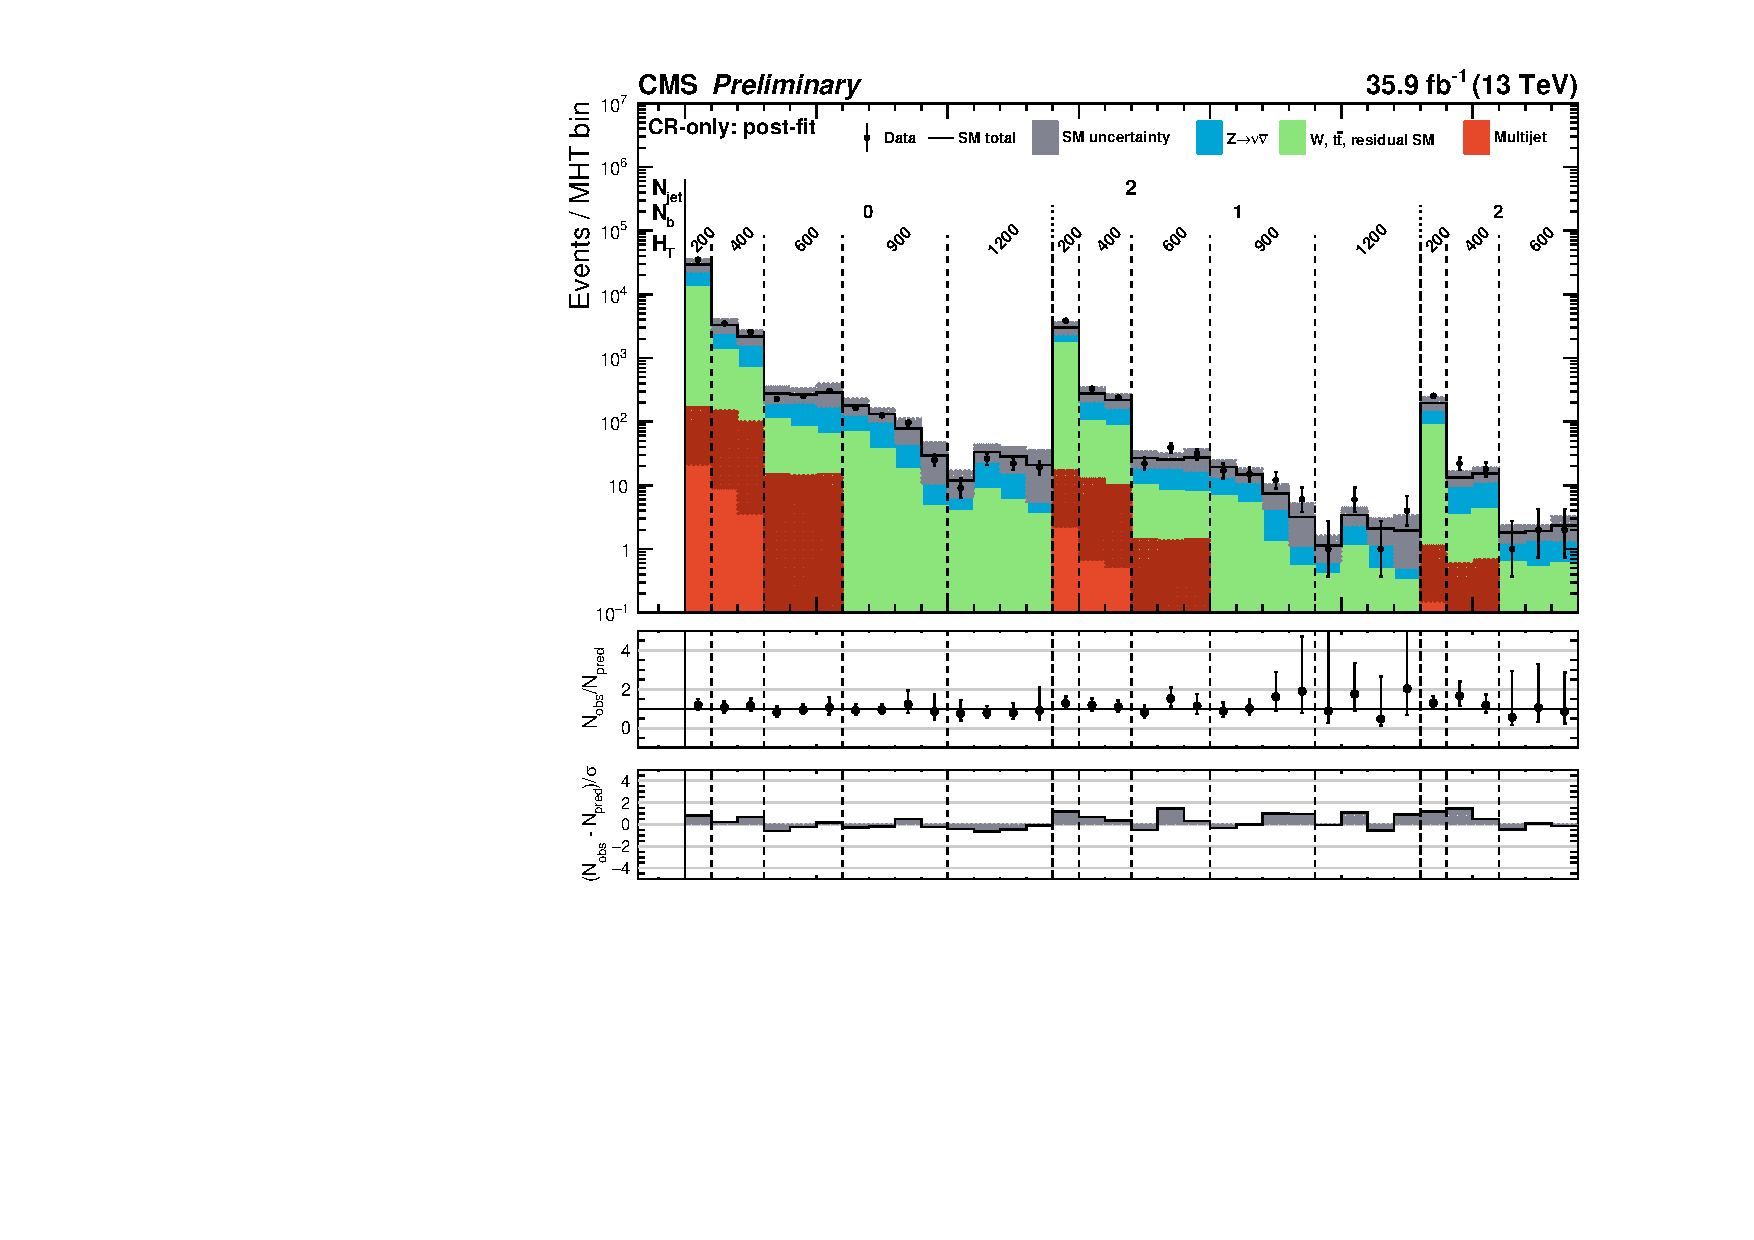
\includegraphics[width=0.48\textwidth]{figures/results/36invfb_preapproval/mht_binned/prefit/di-jet_prefit_dists_true.pdf}
  }\\
  \subfigure[\label{fig:cr-fit:three-jet}Topologies with 3 jets]{
    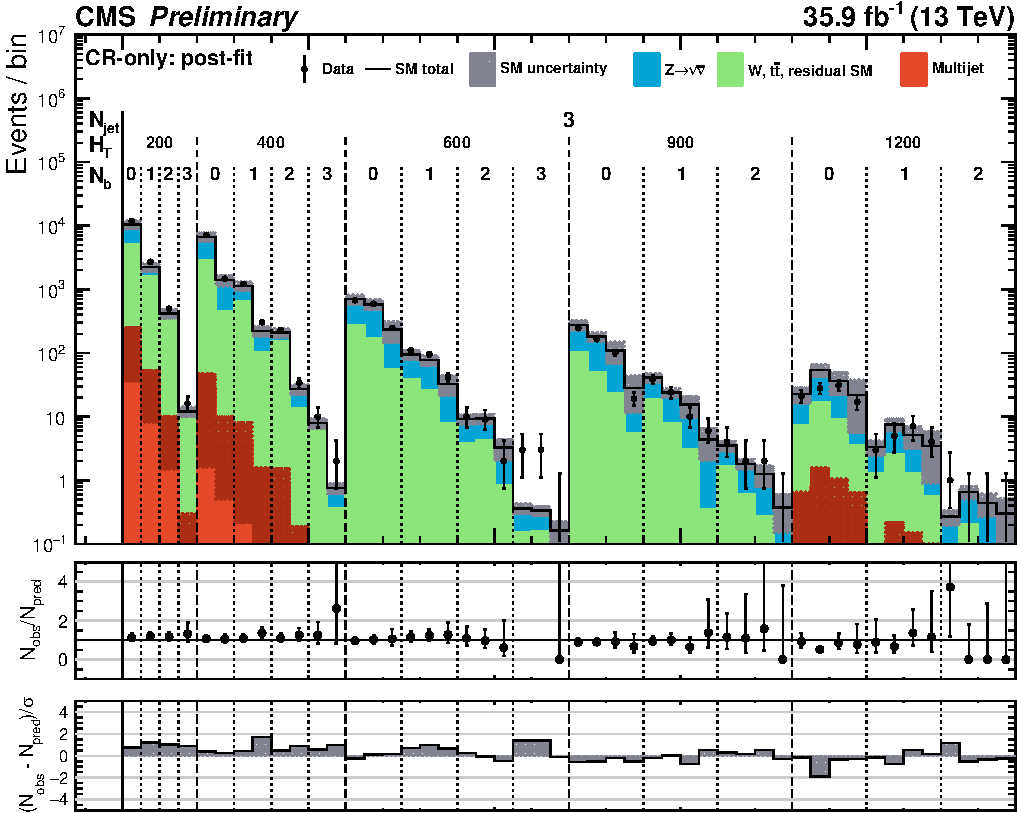
\includegraphics[width=0.48\textwidth]{figures/results/36invfb_preapproval/mht_binned/prefit/3jet_prefit_dists_true.pdf}
  }~ 
  \subfigure[\label{fig:cr-fit:four-jet}Topologies with 4 jets]{
    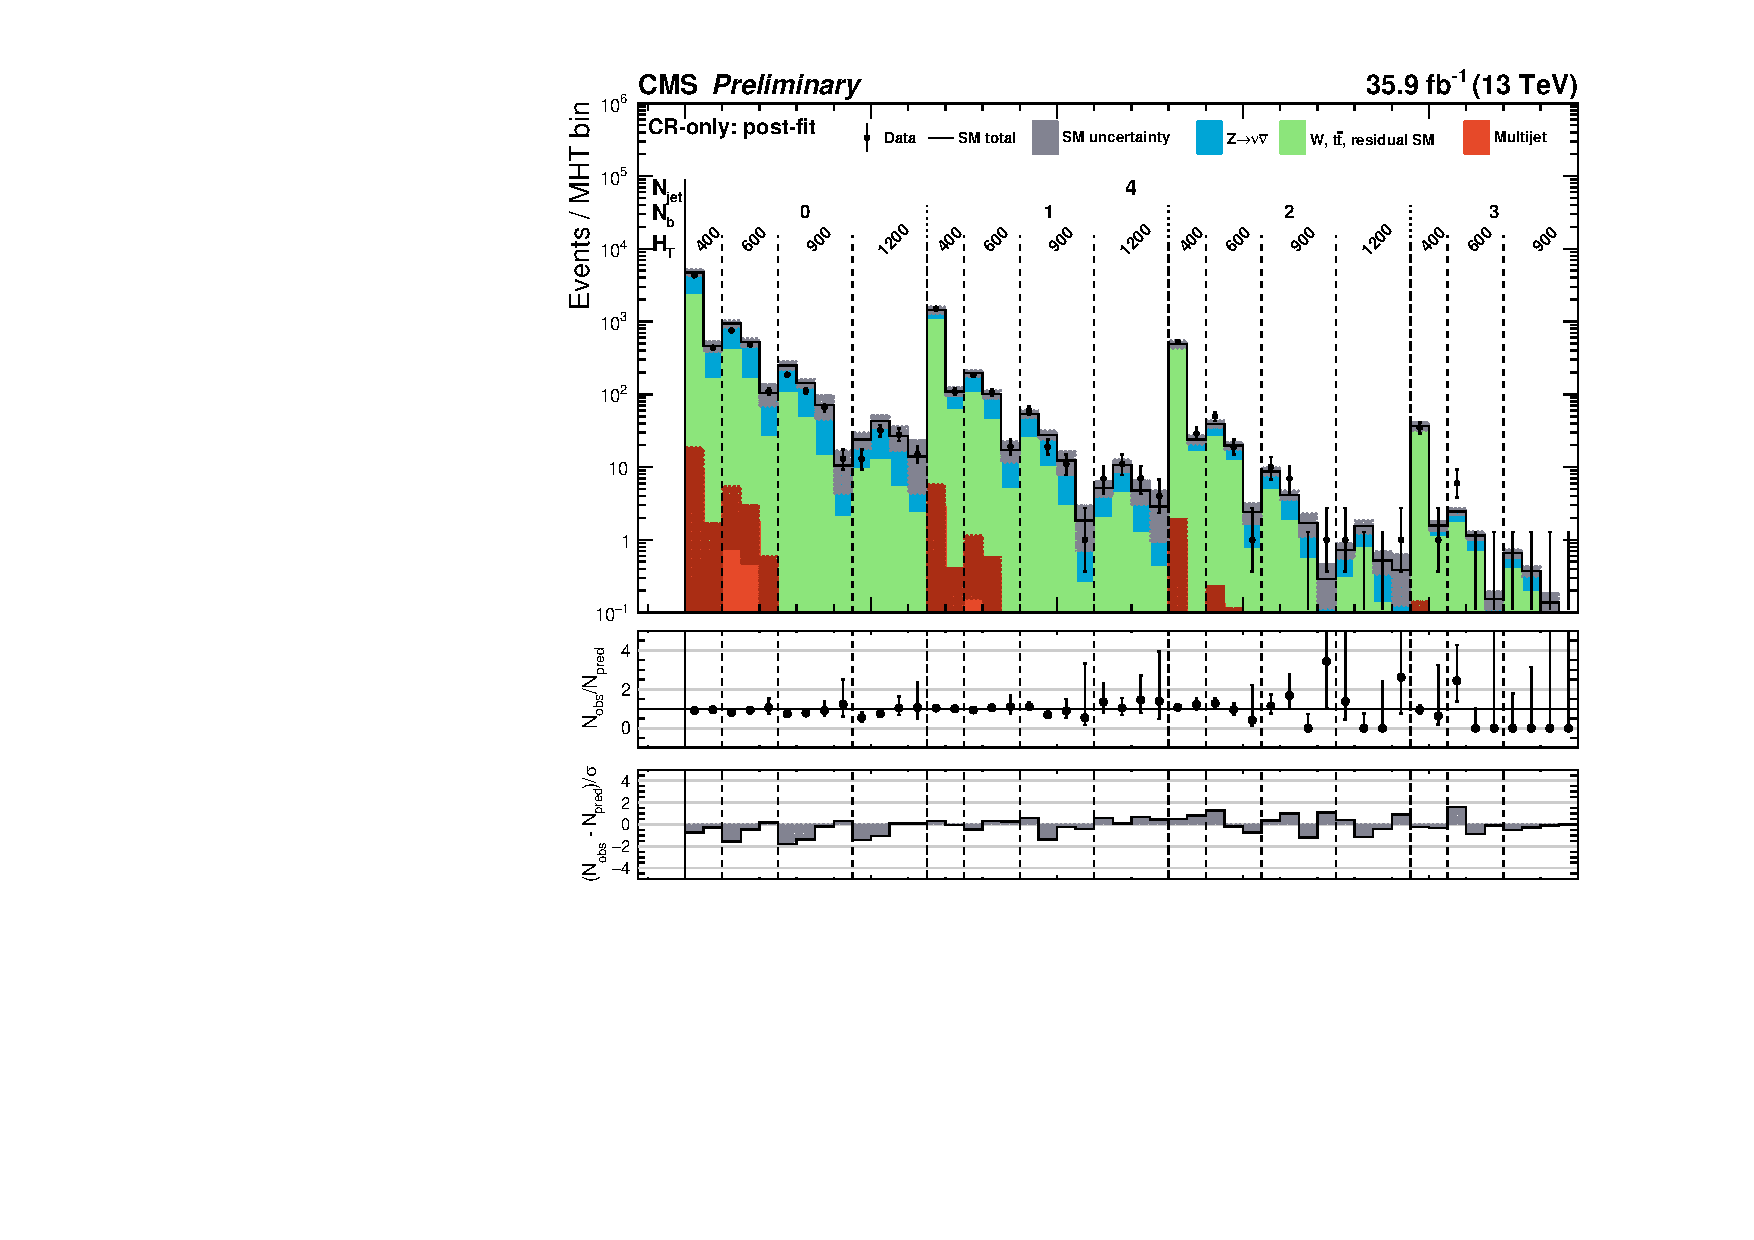
\includegraphics[width=0.48\textwidth]{figures/results/36invfb_preapproval/mht_binned/prefit/4jet_prefit_dists_true.pdf}
  }\\
  \subfigure[\label{fig:cr-fit:five-jet}Topologies with 5 jets]{
    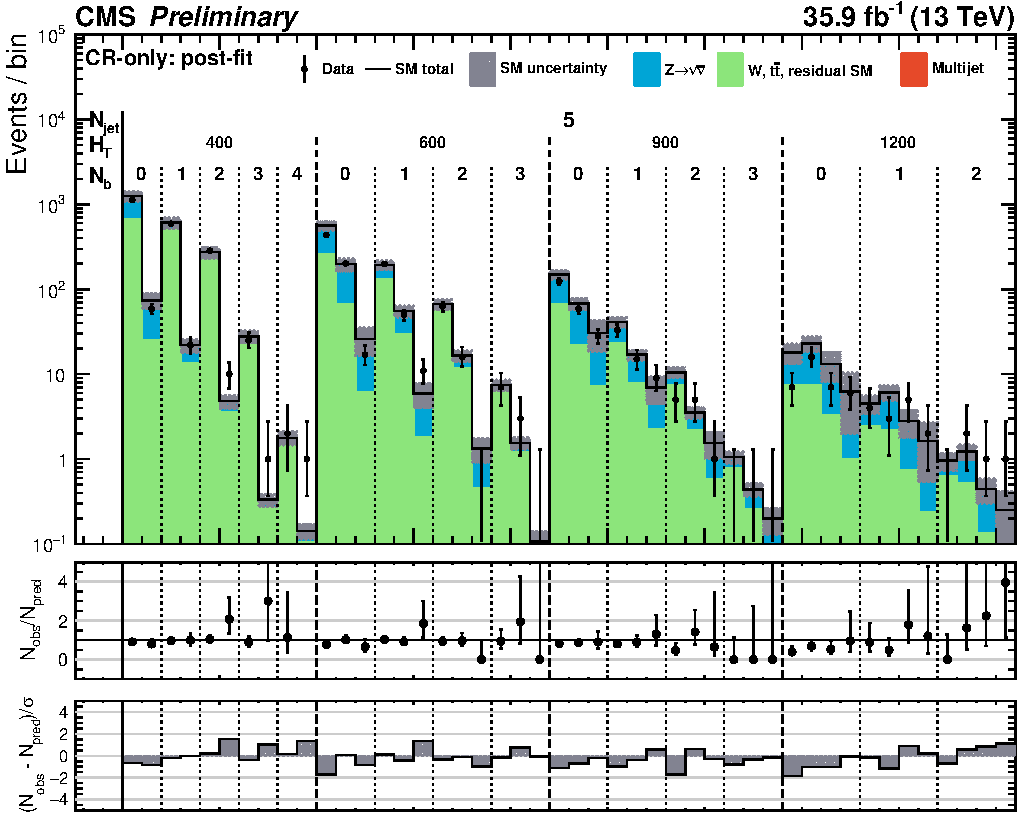
\includegraphics[width=0.48\textwidth]{figures/results/36invfb_preapproval/mht_binned/prefit/5jet_prefit_dists_true.pdf}
  }~ 
  \subfigure[\label{fig:cr-fit:six-jet}Topologies with $\ge$6 jets]{
    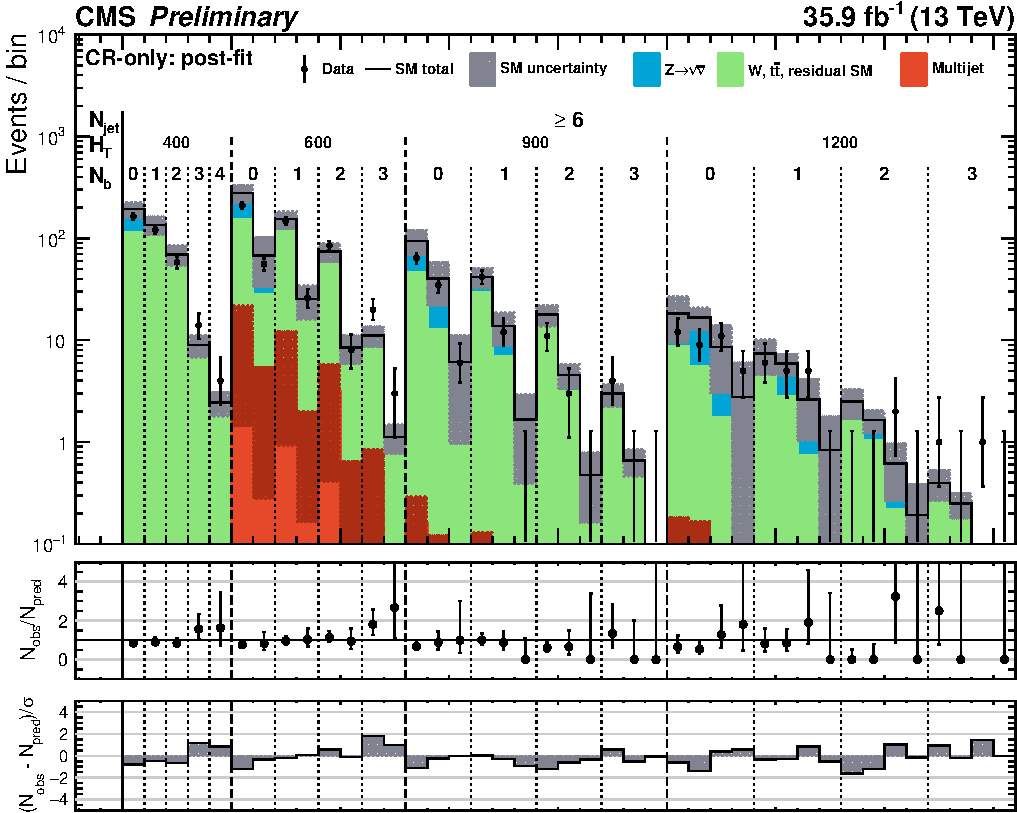
\includegraphics[width=0.48\textwidth]{figures/results/36invfb_preapproval/mht_binned/prefit/6+_jets_prefit_dists_true.pdf}
  }\\
  \caption{\label{fig:cr-fit} Results of the control region-only fit in the 7 different event topologies.
  Top panels:  Event yields in data and SM expectations.
  Centre panels:  Ratio of the observed and expected counts.
  Bottom panels:  Observed pulls of the data from expectation.
  Detailed descriptions are given in the text.
	}
\end{figure}


\clearpage
\begin{figure}[!h]
  \centering
  \subfigure[\label{fig:full-fit:mono-asymm}Monojet and asymmetric topologies]{
    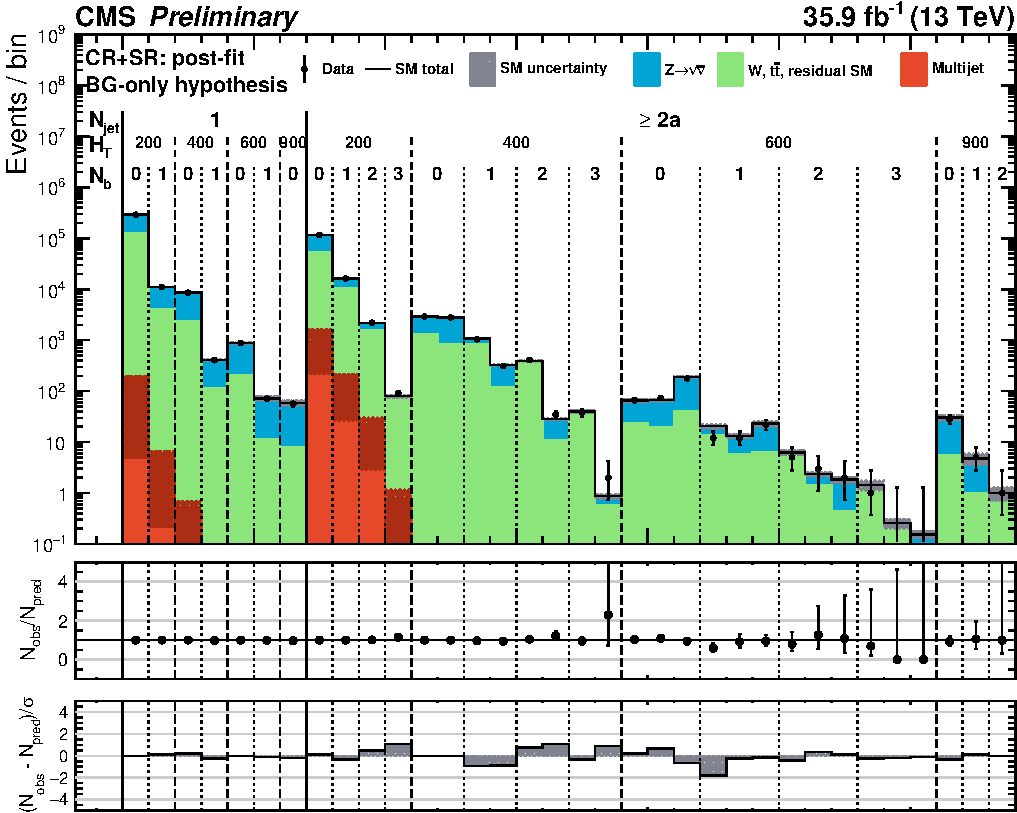
\includegraphics[width=0.48\textwidth]{figures/results/36invfb_preapproval/mht_binned/fit_b/monojet_fit_b_dists_true.pdf}
  }~ 
  \subfigure[\label{fig:full-fit:dijet}Dijet topologies]{
    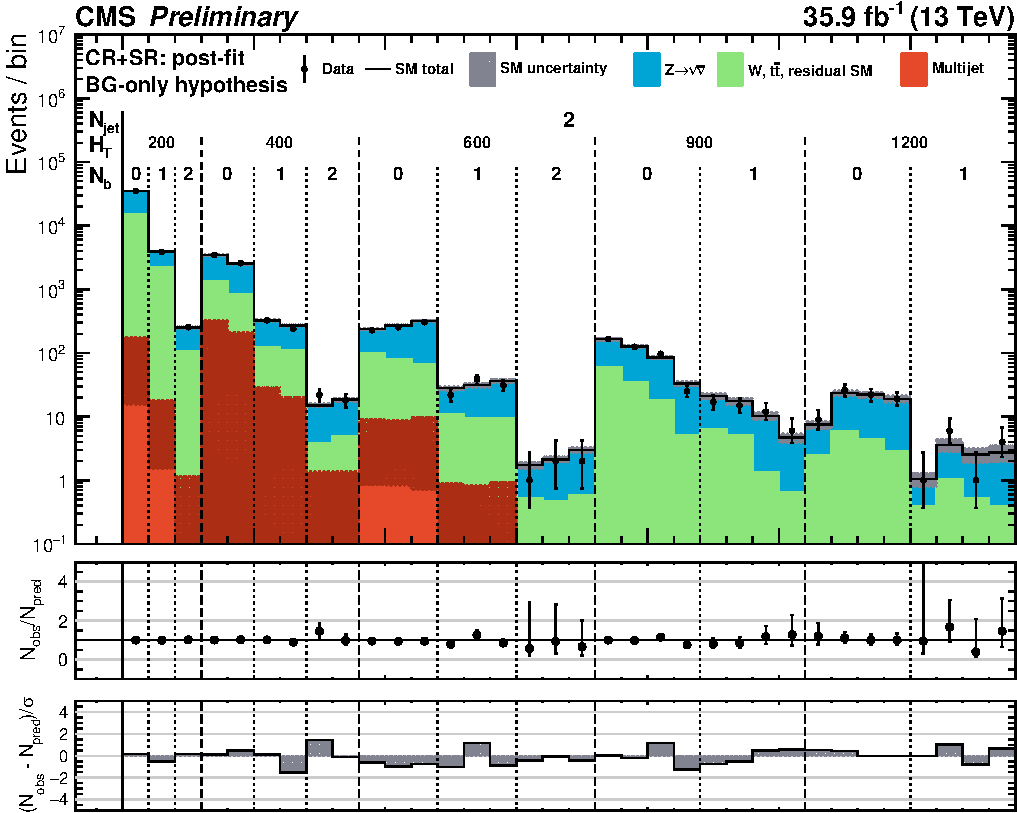
\includegraphics[width=0.48\textwidth]{figures/results/36invfb_preapproval/mht_binned/fit_b/di-jet_fit_b_dists_true.pdf}
  }\\
  \subfigure[\label{fig:full-fit:three-jet}Topologies with 3 jets]{
    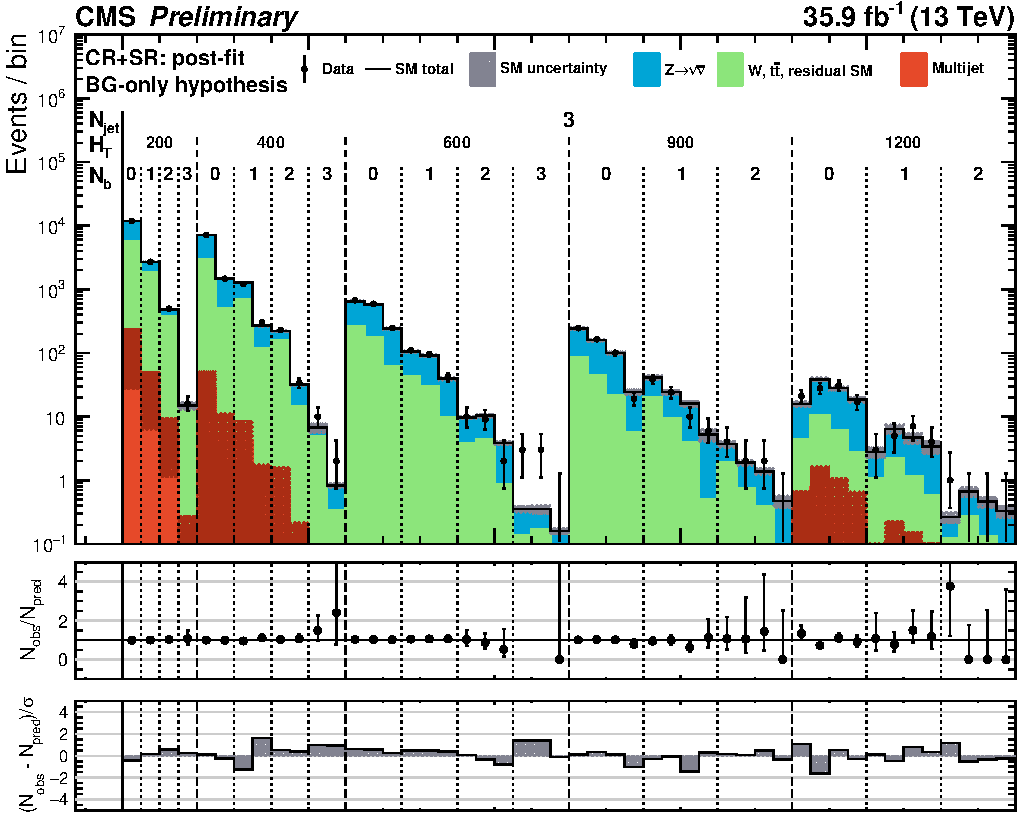
\includegraphics[width=0.48\textwidth]{figures/results/36invfb_preapproval/mht_binned/fit_b/3jet_fit_b_dists_true.pdf}
  }~ 
  \subfigure[\label{fig:full-fit:four-jet}Topologies with 4 jets]{
    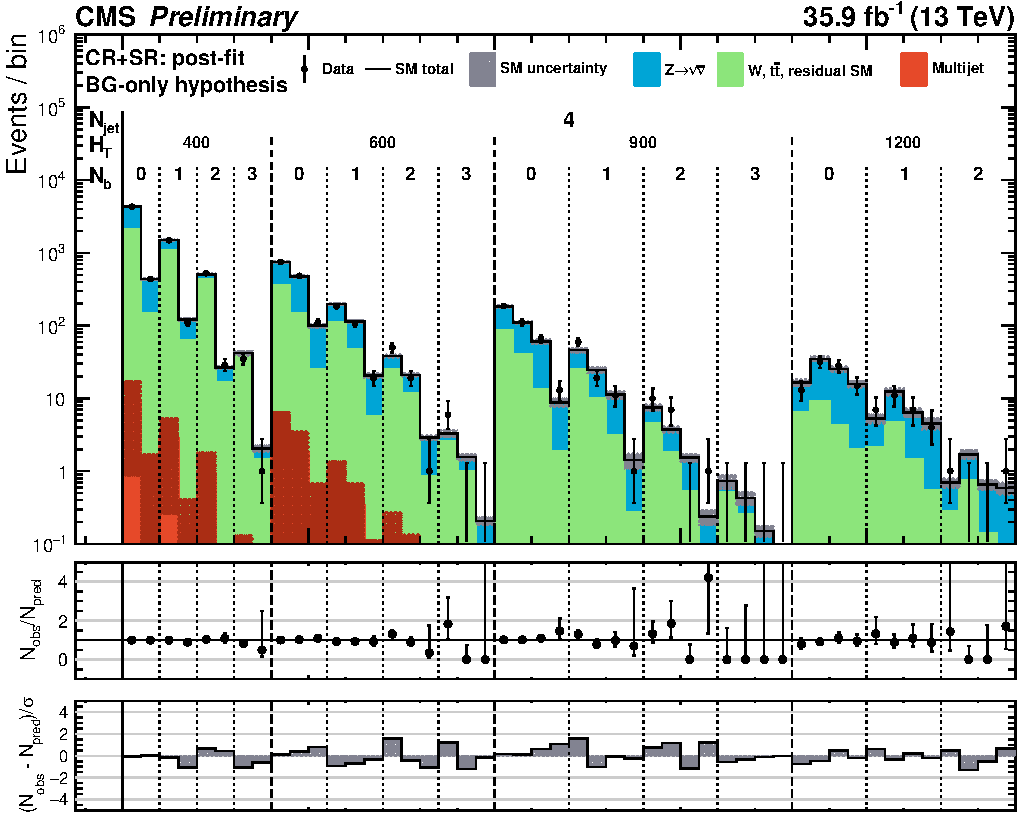
\includegraphics[width=0.48\textwidth]{figures/results/36invfb_preapproval/mht_binned/fit_b/4jet_fit_b_dists_true.pdf}
  }\\
  \subfigure[\label{fig:full-fit:five-jet}Topologies with 5 jets]{
    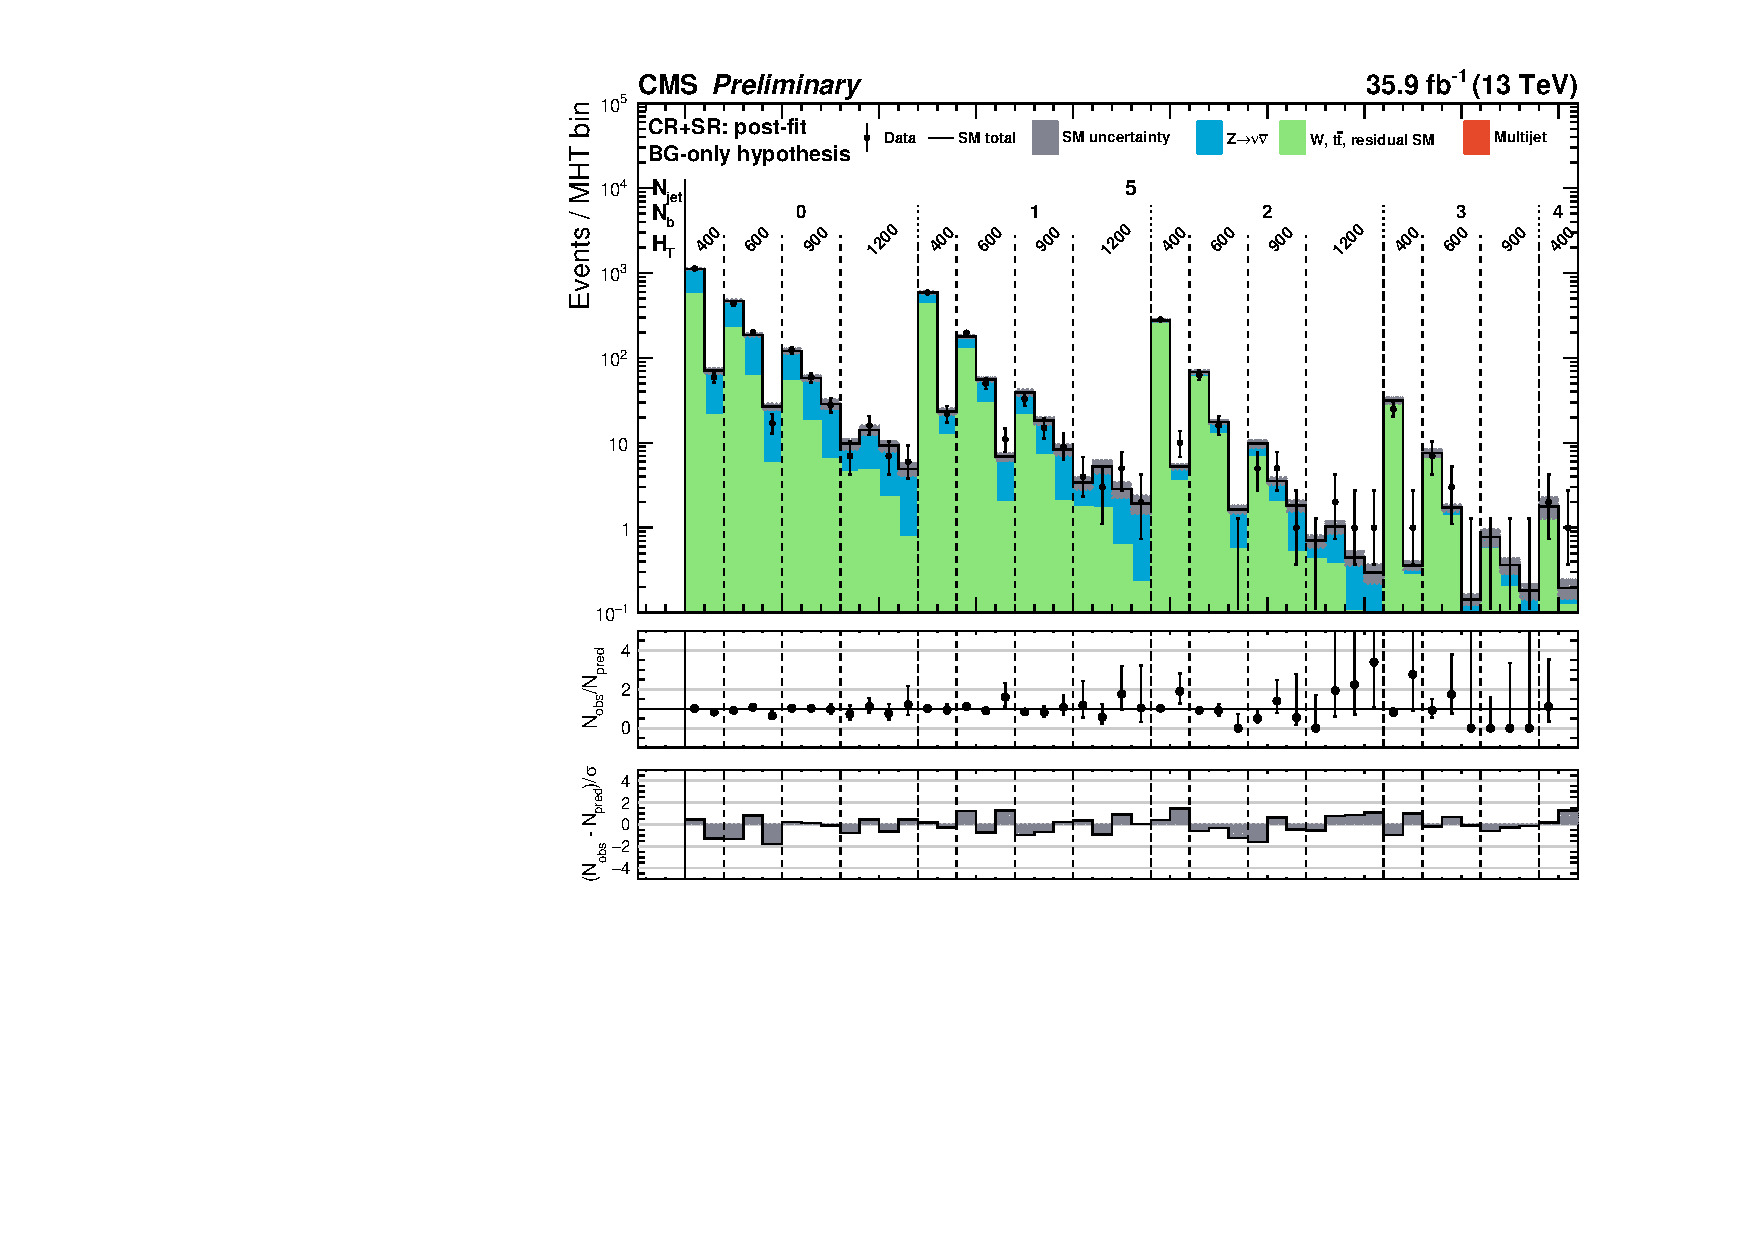
\includegraphics[width=0.48\textwidth]{figures/results/36invfb_preapproval/mht_binned/fit_b/5jet_fit_b_dists_true.pdf}
  }~ 
  \subfigure[\label{fig:full-fit:six-jet}Topologies with $\ge$6 jets]{
    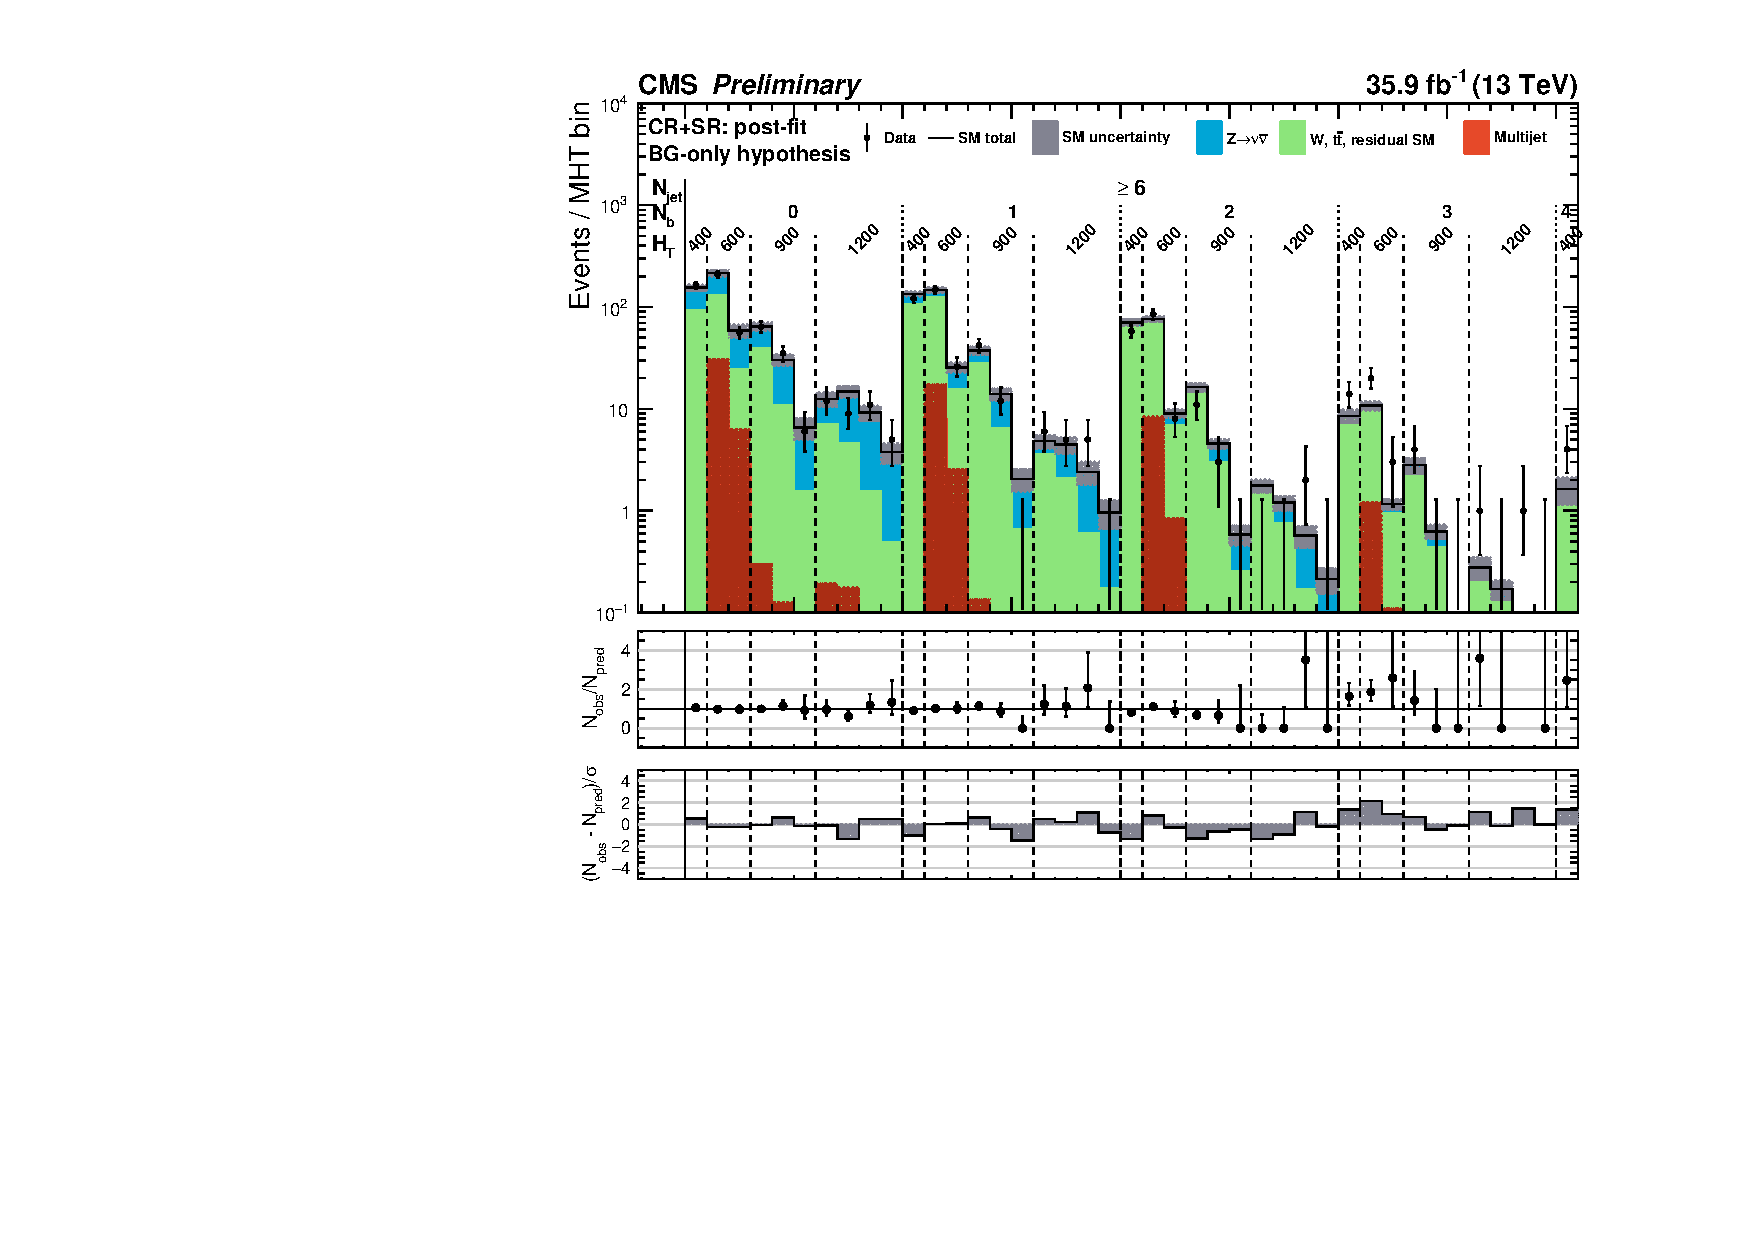
\includegraphics[width=0.48\textwidth]{figures/results/36invfb_preapproval/mht_binned/fit_b/6+_jets_fit_b_dists_true.pdf}
  }\\
  \caption{\label{fig:full-fit} Results of the full fit in the 7 different event topologies.
  Top panels:  Event yields in data and SM expectations.
  Centre panels:  Ratio of the observed and expected counts.
  Bottom panels:  Observed pulls of the data from expectation.
  Detailed descriptions are given in the text.
	}
\end{figure}

%% mono 
%\clearpage
%\subsection{Monojet topology}
%
%\begin{figure}[h!]
%  \centering
%  \caption{Upper panel. Event yields observed in data (solid circles)
%    and SM expectations with their associated uncertainties (black
%    histogram with shaded band) as a function of \nb and \scalht,
%    integrated over \mht, and for the monojet category ($\njet = 1$)
%    in the signal region. Lower panel. Data-to-background ratios. The
%    background estimates and ratios are from the masked fit. }
%  \label{fig:mr_mono_pre}
%  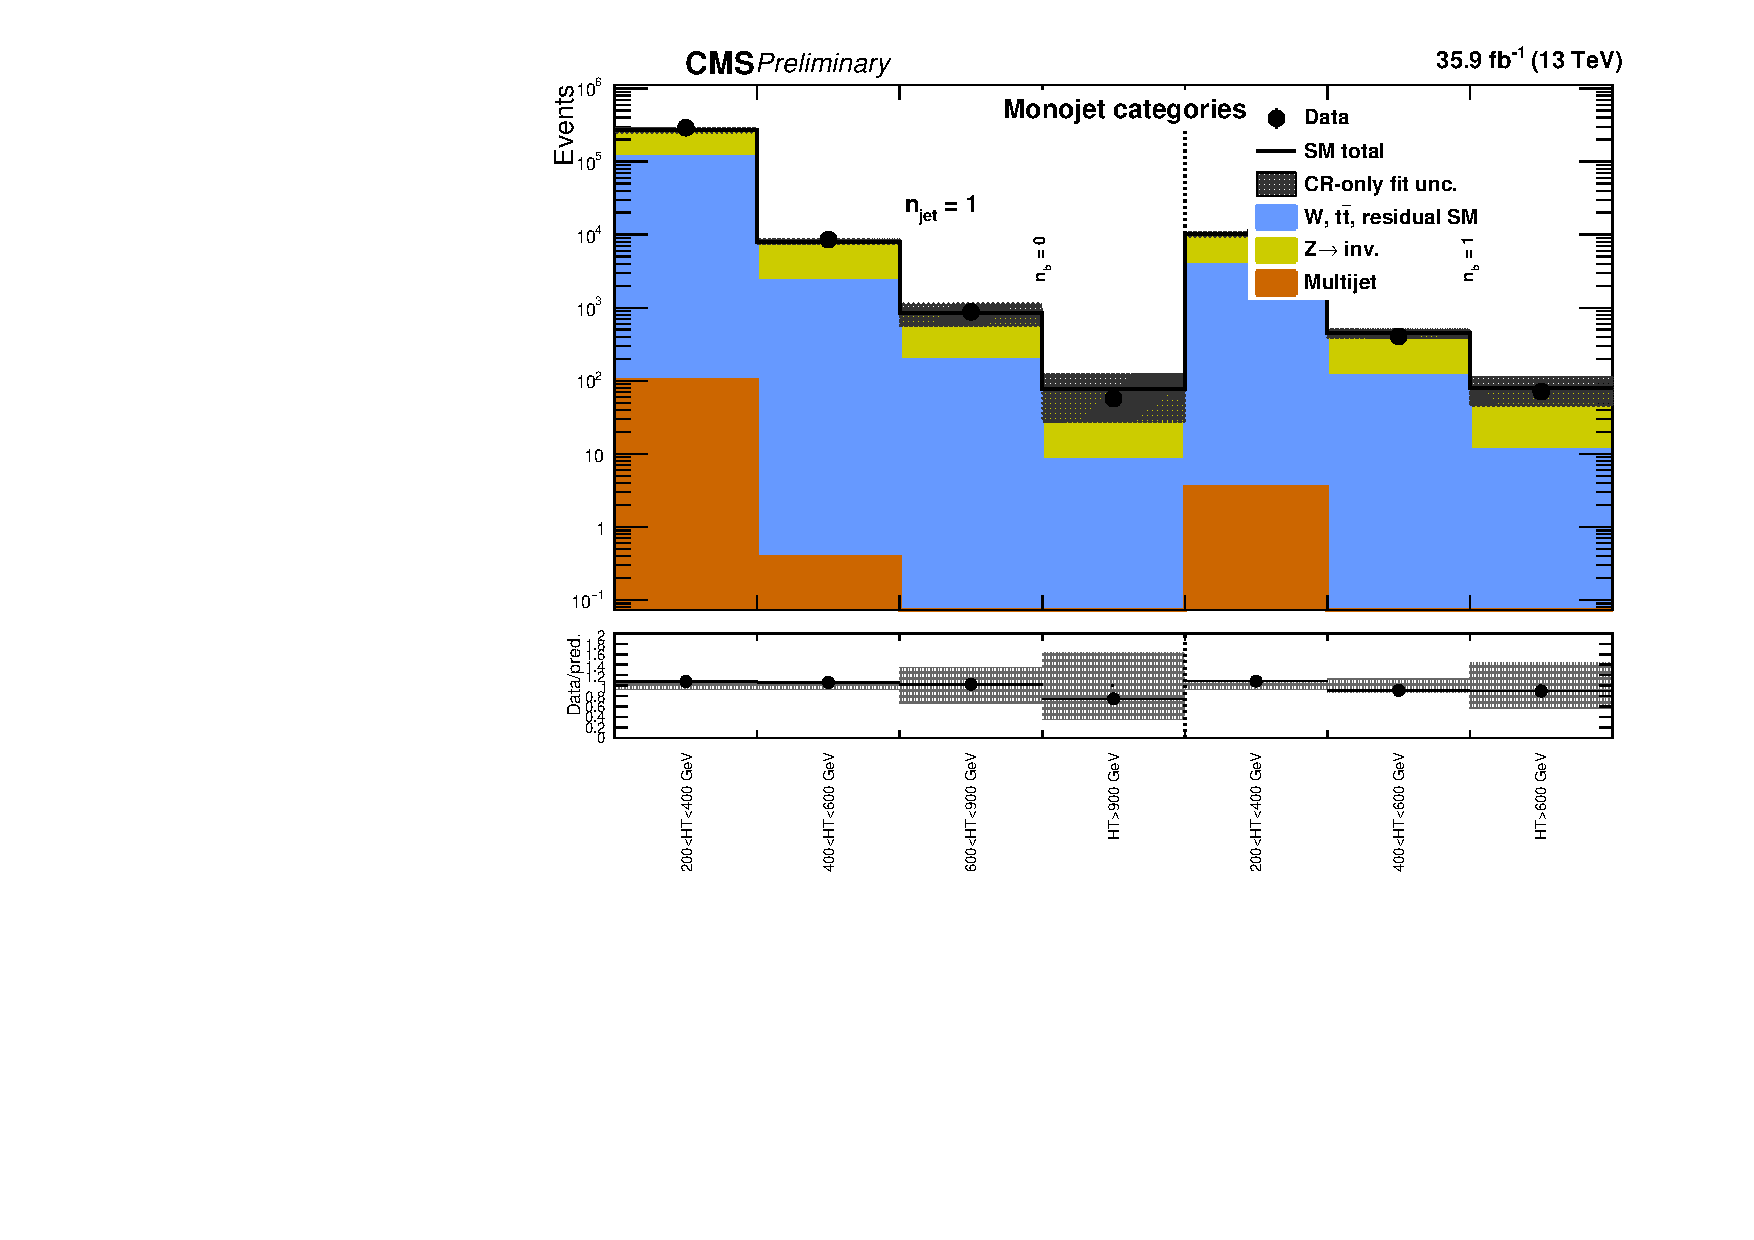
\includegraphics[width=1.\linewidth]{figures/results/36invfb_preapproval/mono/summaryPlot_Monojet_prefit}
%\end{figure}
%
%\clearpage
%\begin{figure}[h!]
%  \centering
%  \caption{Upper panel. Event yields observed in data (solid circles)
%    and SM expectations with their associated uncertainties (black
%    histogram with shaded band) as a function of \nb and \scalht,
%    integrated over \mht, and for the monojet category ($\njet = 1$)
%    in the signal region. Lower panel. Data-to-background ratios. The
%    background estimates and ratios are obtained with the full fit. }
%  \label{fig:mr_mono_post}
%  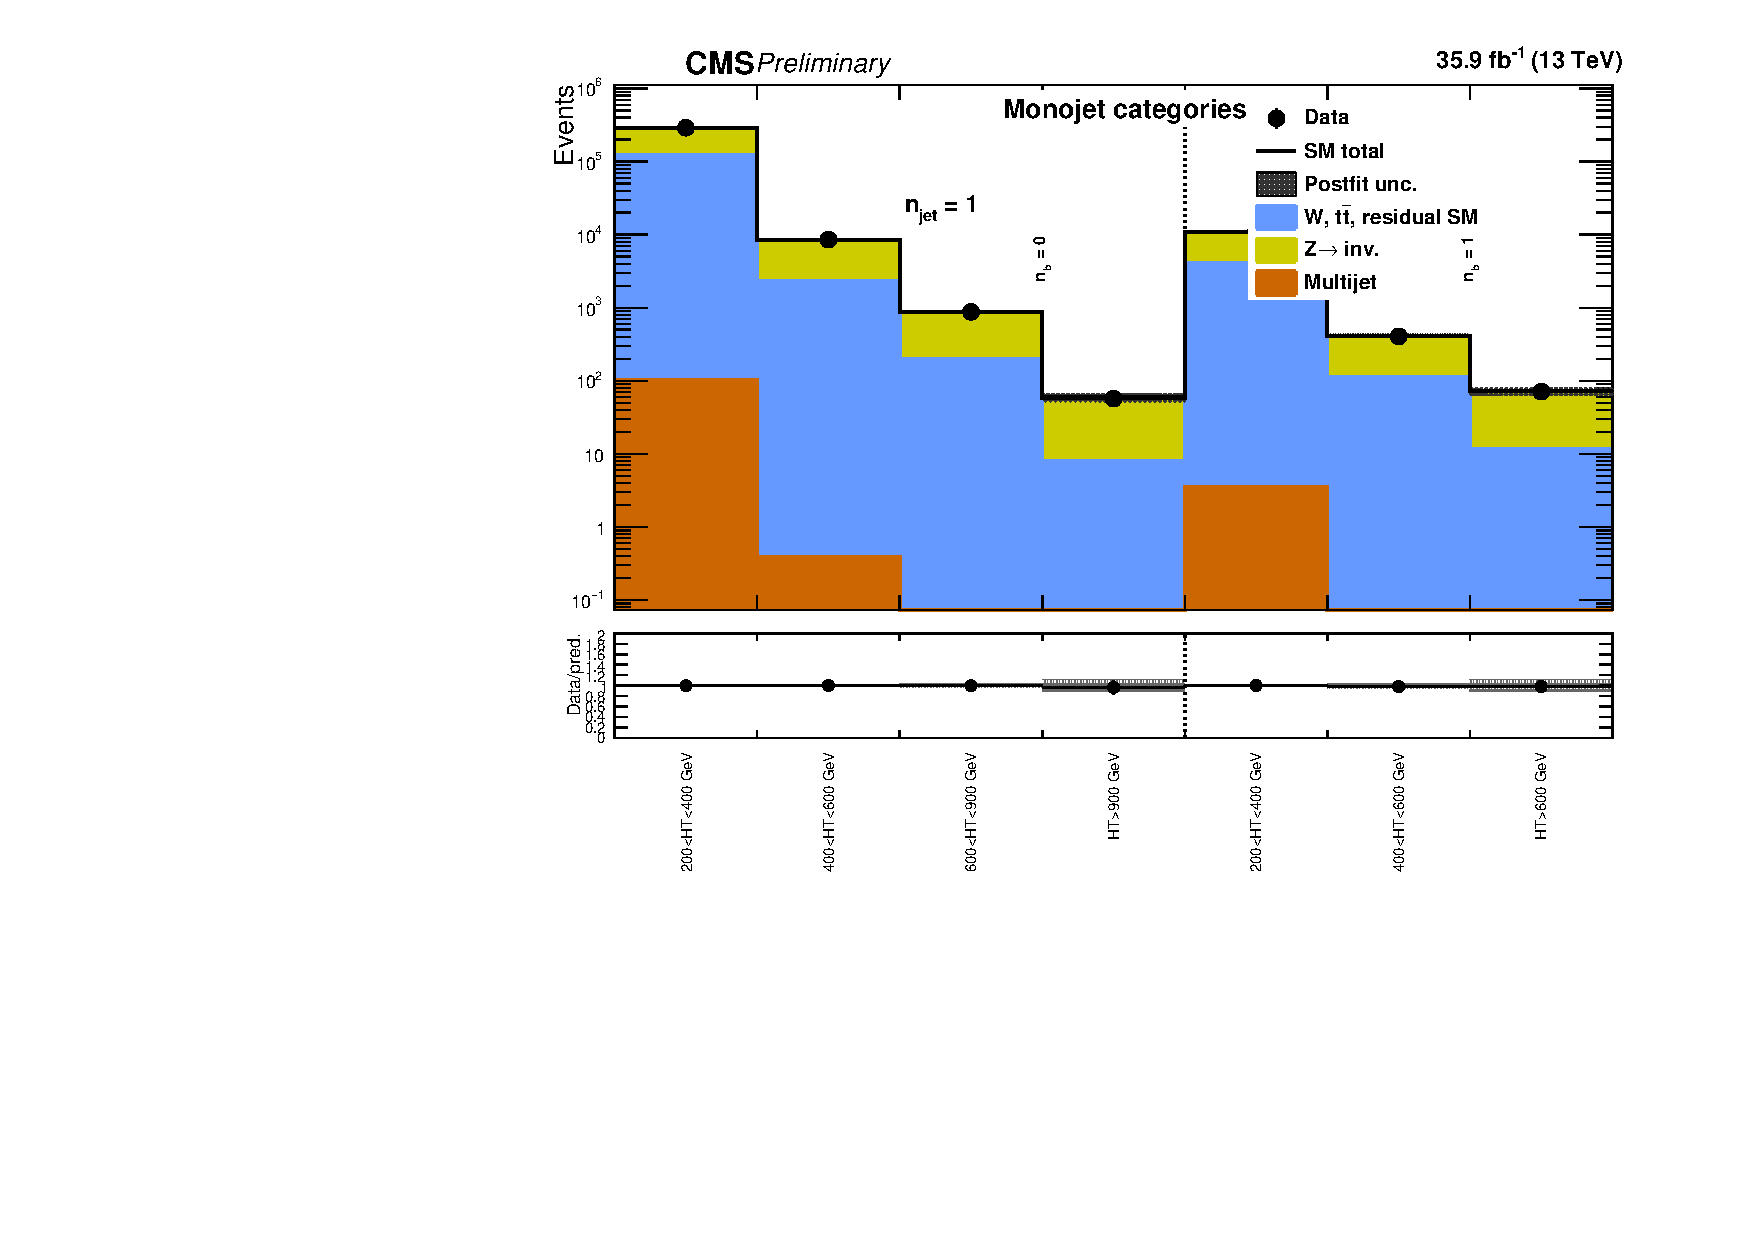
\includegraphics[width=1.\linewidth]{figures/results/36invfb_preapproval/mono/summaryPlot_Monojet_fit_b}
%\end{figure}
%
%\clearpage
%\begin{figure}[h!]
%  \centering
%  \caption{Upper panel. Event yields observed in data (solid circles)
%    and SM expectations with their associated uncertainties (black
%    histogram with shaded band) as a function of \nb and \scalht,
%    integrated over \mht, and for the monojet category ($\njet = 1$)
%    in the signal region. Lower panel. The pulls, which are obtained
%    from both the masked (red markers) and full (blue markers) fits. }
%  \label{fig:mr_mono_pulls}
%  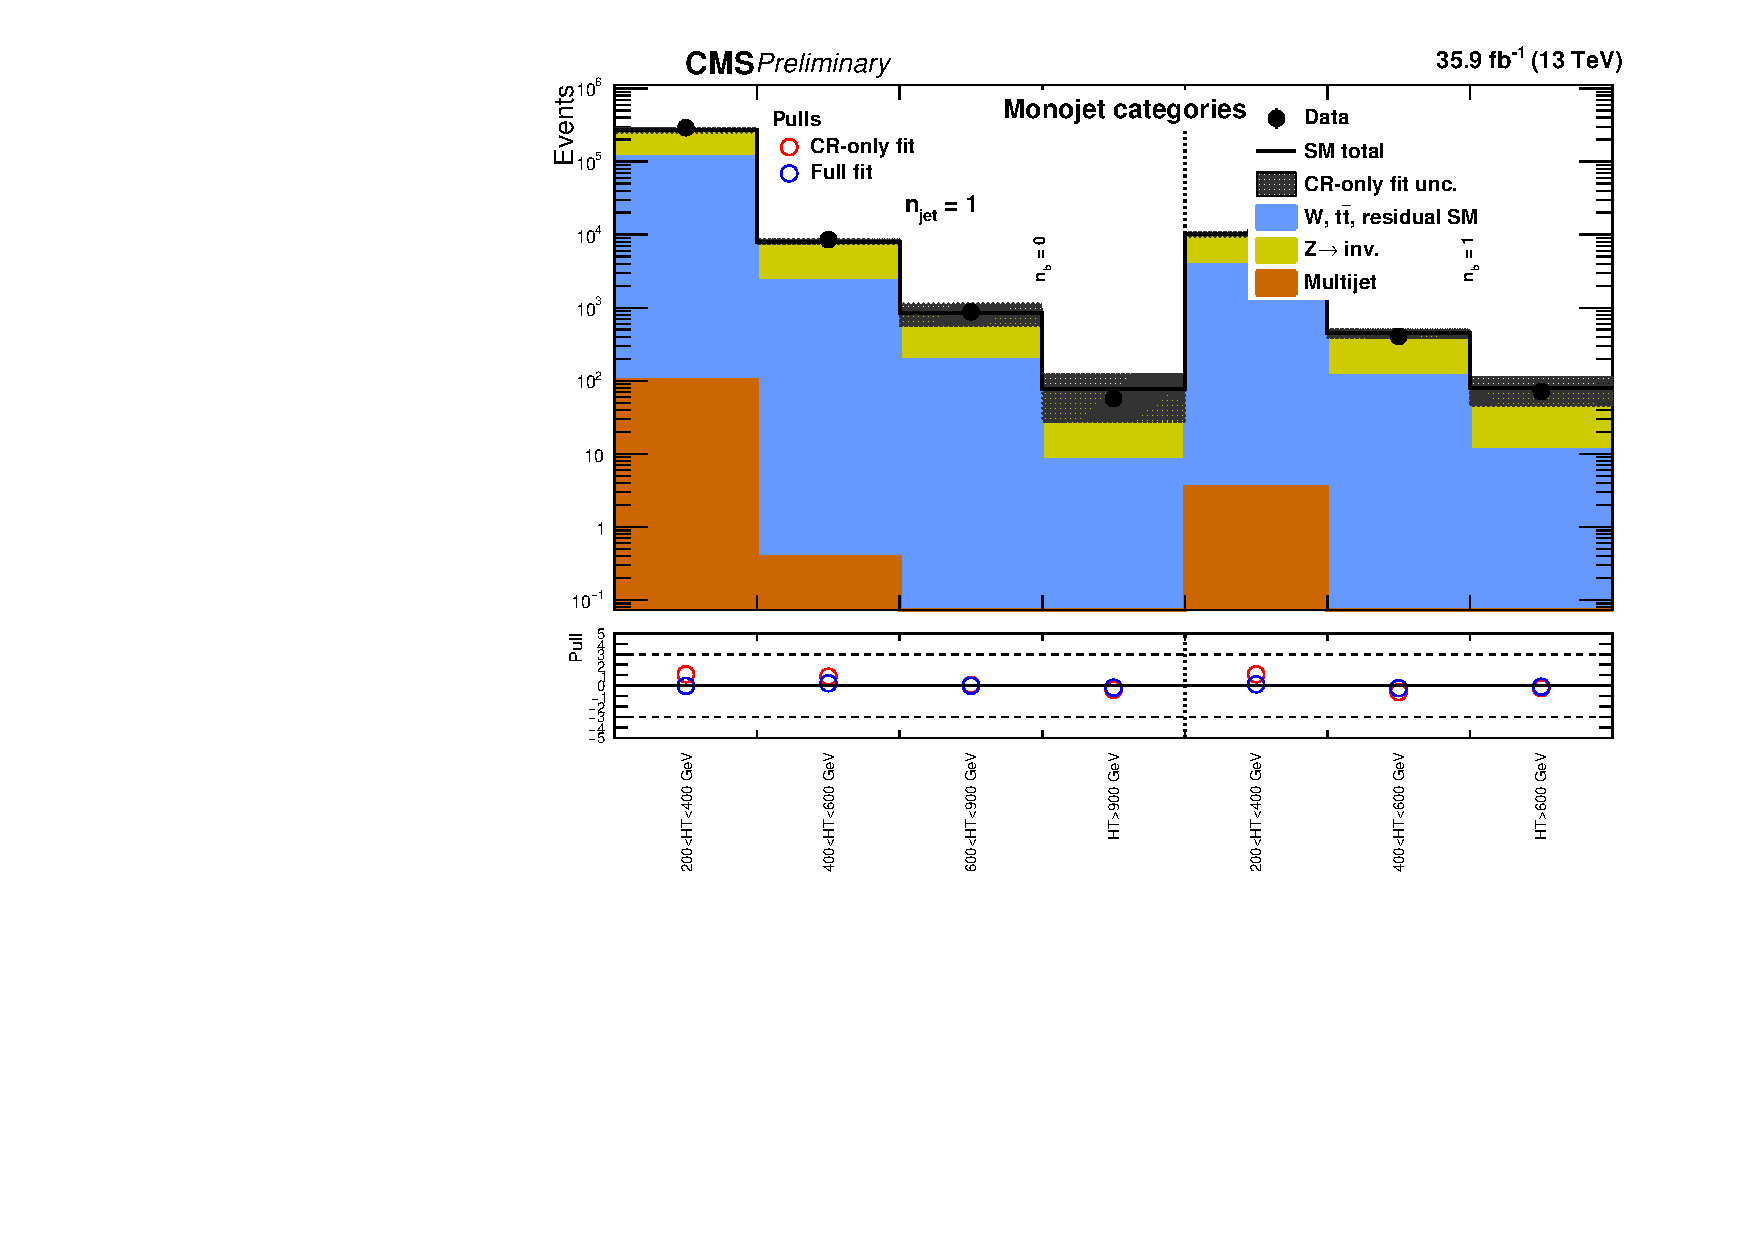
\includegraphics[width=1.\linewidth]{figures/results/36invfb_preapproval/mono/summaryPlot_Monojet_prefit_overlay_fit_b}
%\end{figure}
%
%% asym 
%\clearpage
%\subsection{Asymmetric topology}
%
%\begin{figure}[h!]
%  \centering
%  \caption{Upper panel. Event yields observed in data (solid circles)
%    and SM expectations with their associated uncertainties (black
%    histogram with shaded band) as a function of \nb and \scalht,
%    integrated over \mht, and for the asymmetric \njet category
%    in the signal region. Lower panel. Data-to-background ratios. The
%    background estimates and ratios are from the masked fit. }
%  \label{fig:mr_asym_pre}
%  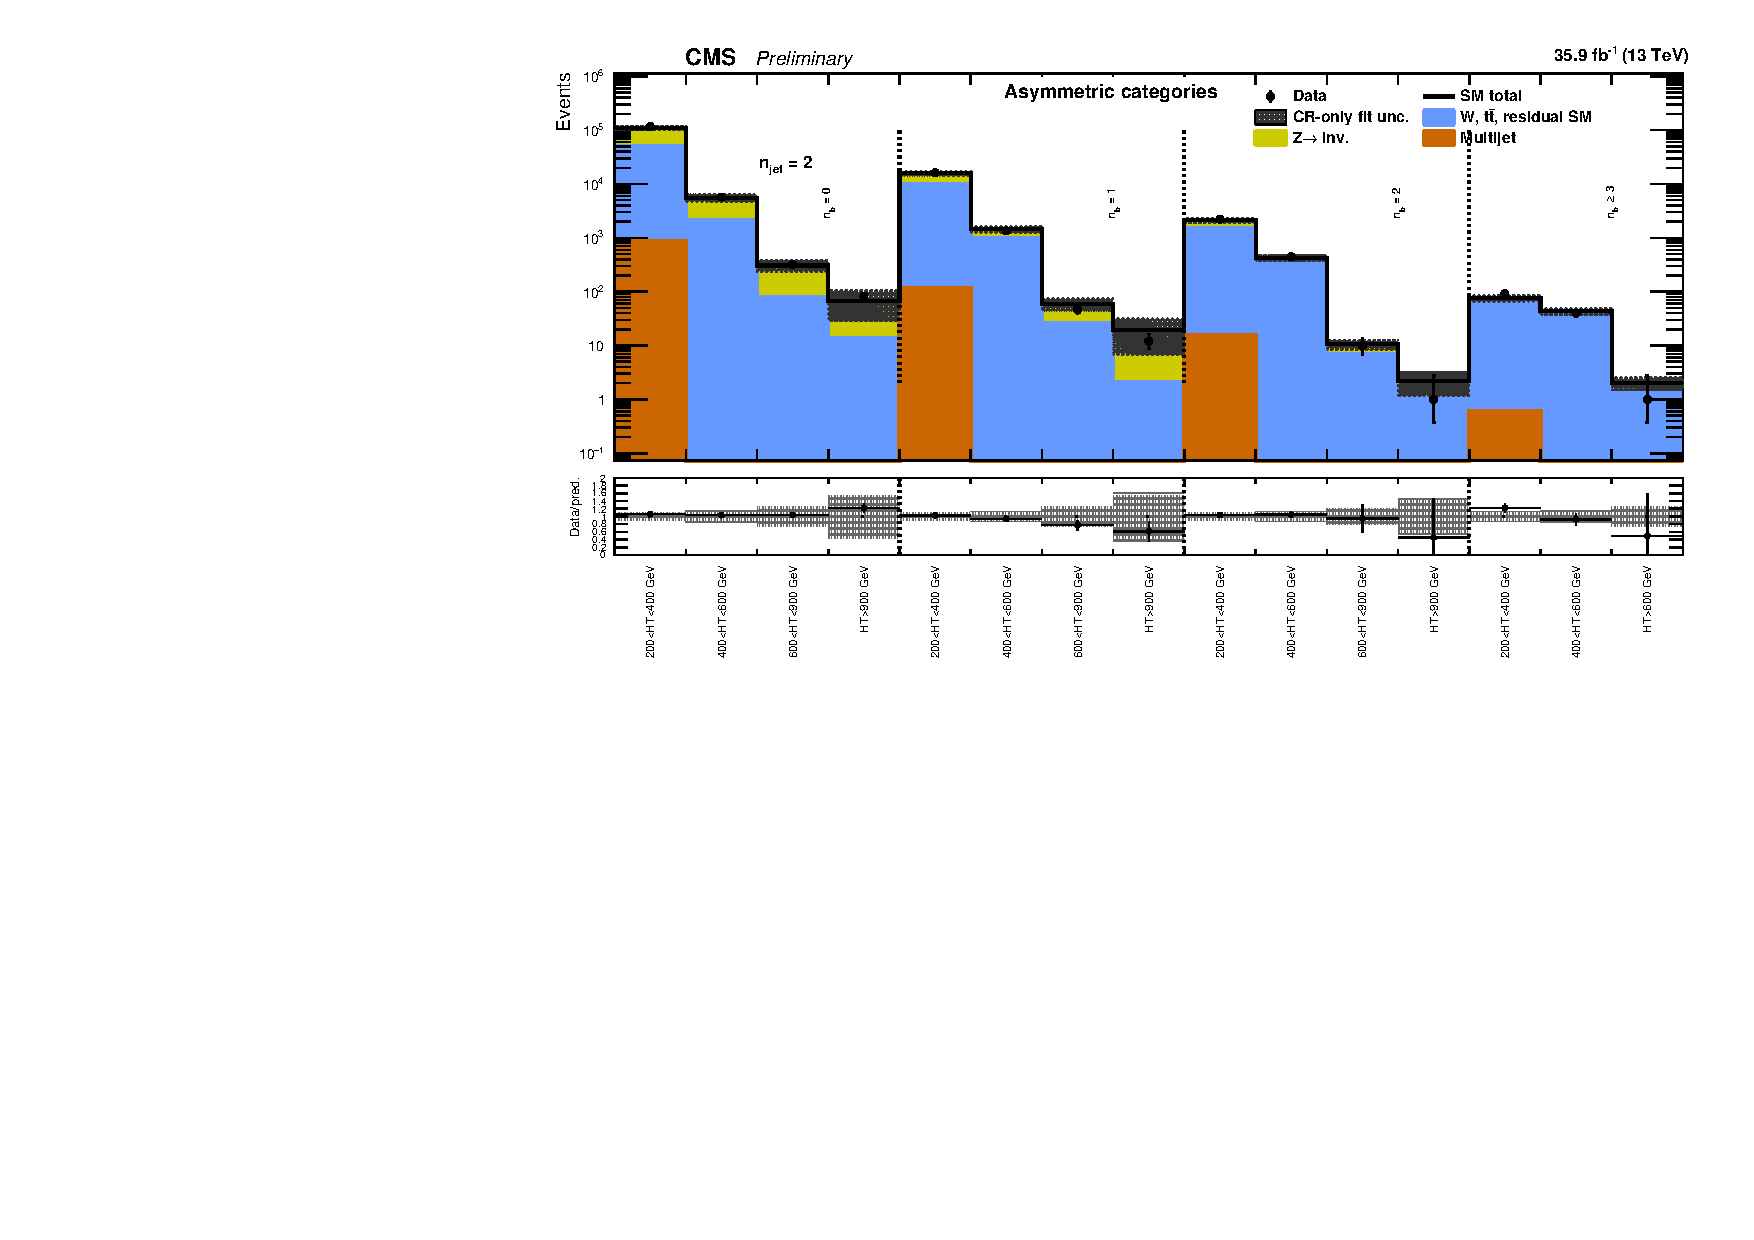
\includegraphics[width=1.\linewidth]{figures/results/36invfb_preapproval/asym/summaryPlot_Asymmetric_prefit}
%\end{figure}
%
%\clearpage
%\begin{figure}[h!]
%  \centering
%  \caption{Upper panel. Event yields observed in data (solid circles)
%    and SM expectations with their associated uncertainties (black
%    histogram with shaded band) as a function of \nb and \scalht,
%    integrated over \mht, and for the asymmetric \njet category
%    in the signal region. Lower panel. Data-to-background ratios. The
%    background estimates and ratios are obtained with the full fit. }
%  \label{fig:mr_asym_post}
%  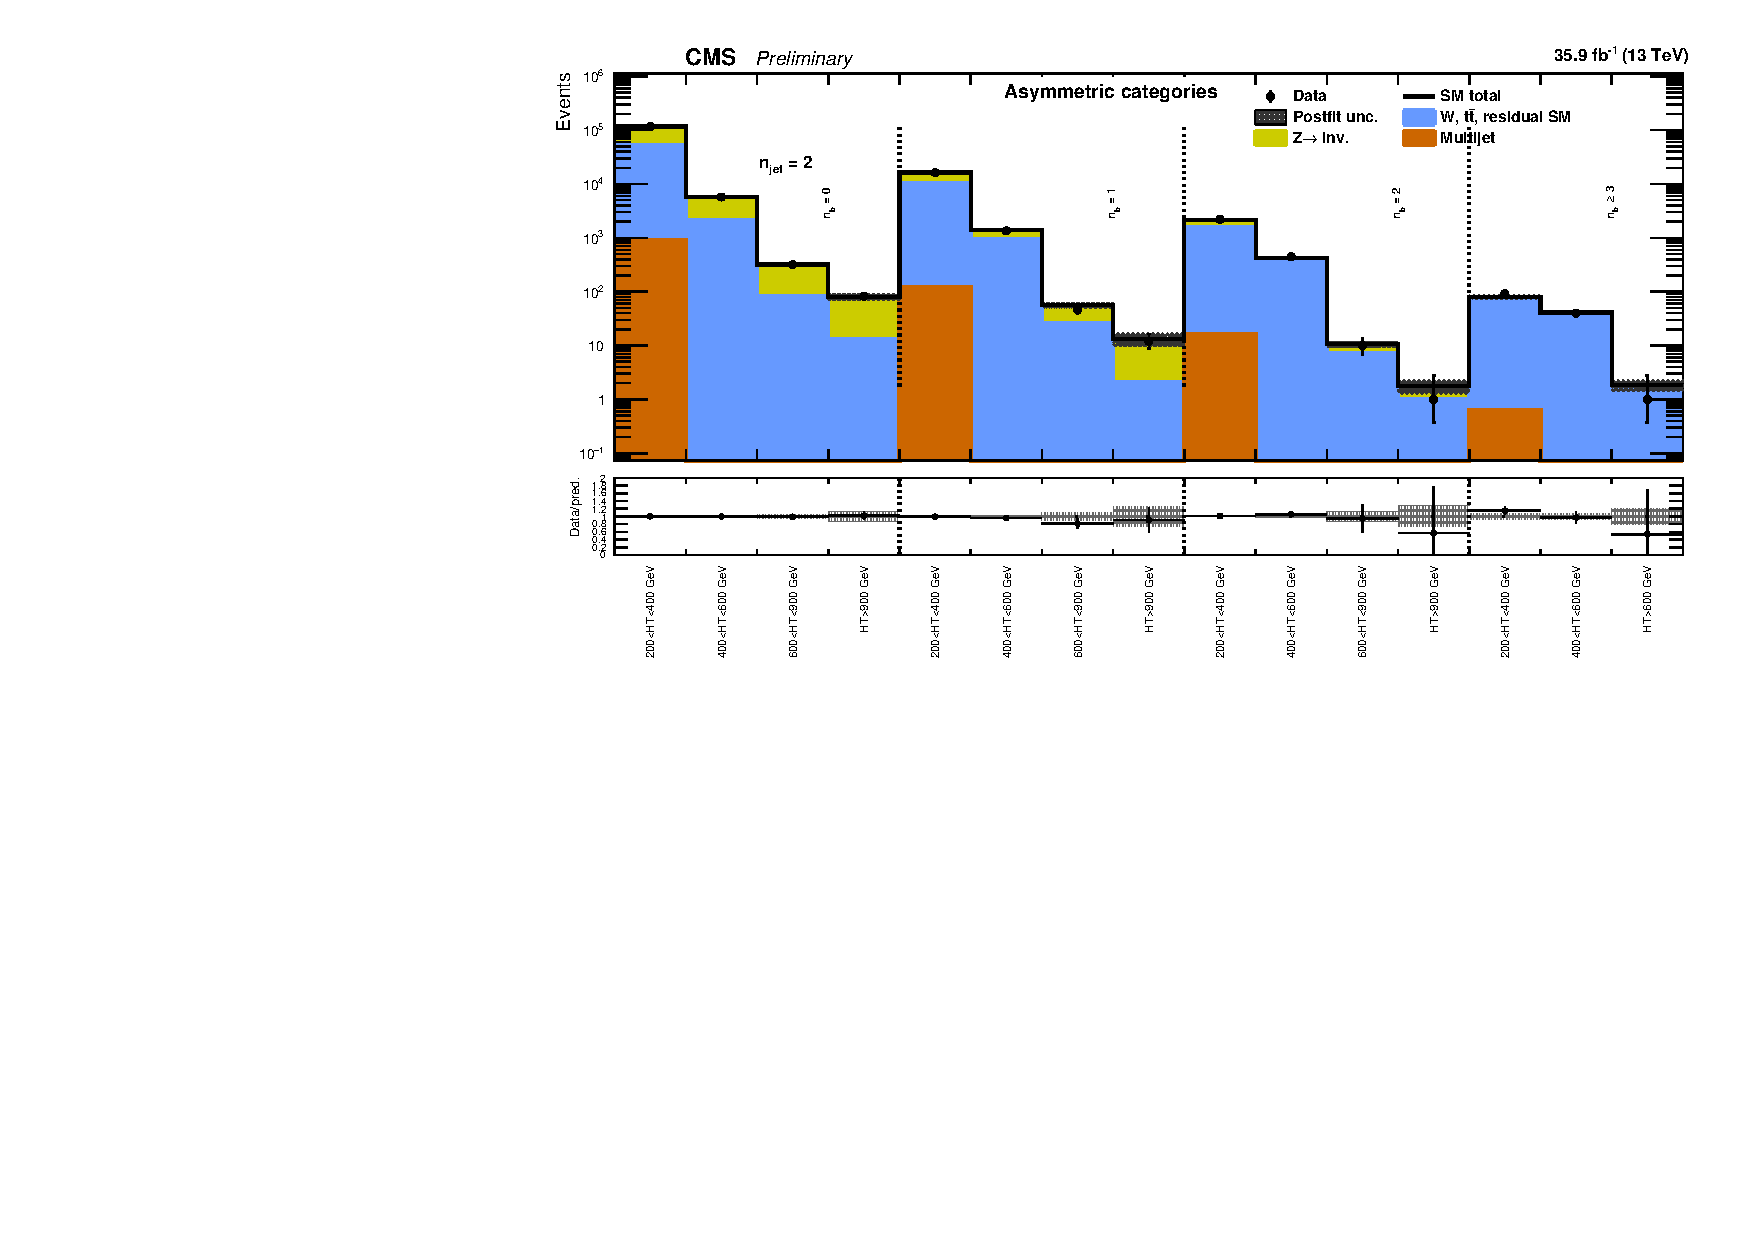
\includegraphics[width=1.\linewidth]{figures/results/36invfb_preapproval/asym/summaryPlot_Asymmetric_fit_b}
%\end{figure}
%
%\clearpage
%\begin{figure}[h!]
%  \centering
%  \caption{Upper panel. Event yields observed in data (solid circles)
%    and SM expectations with their associated uncertainties (black
%    histogram with shaded band) as a function of \nb and \scalht,
%    integrated over \mht, and for the asymmetric \njet category
%    in the signal region. Lower panel. The pulls, which are obtained
%    from both the masked (red markers) and full (blue markers) fits. }
%  \label{fig:mr_asym_pulls}
%  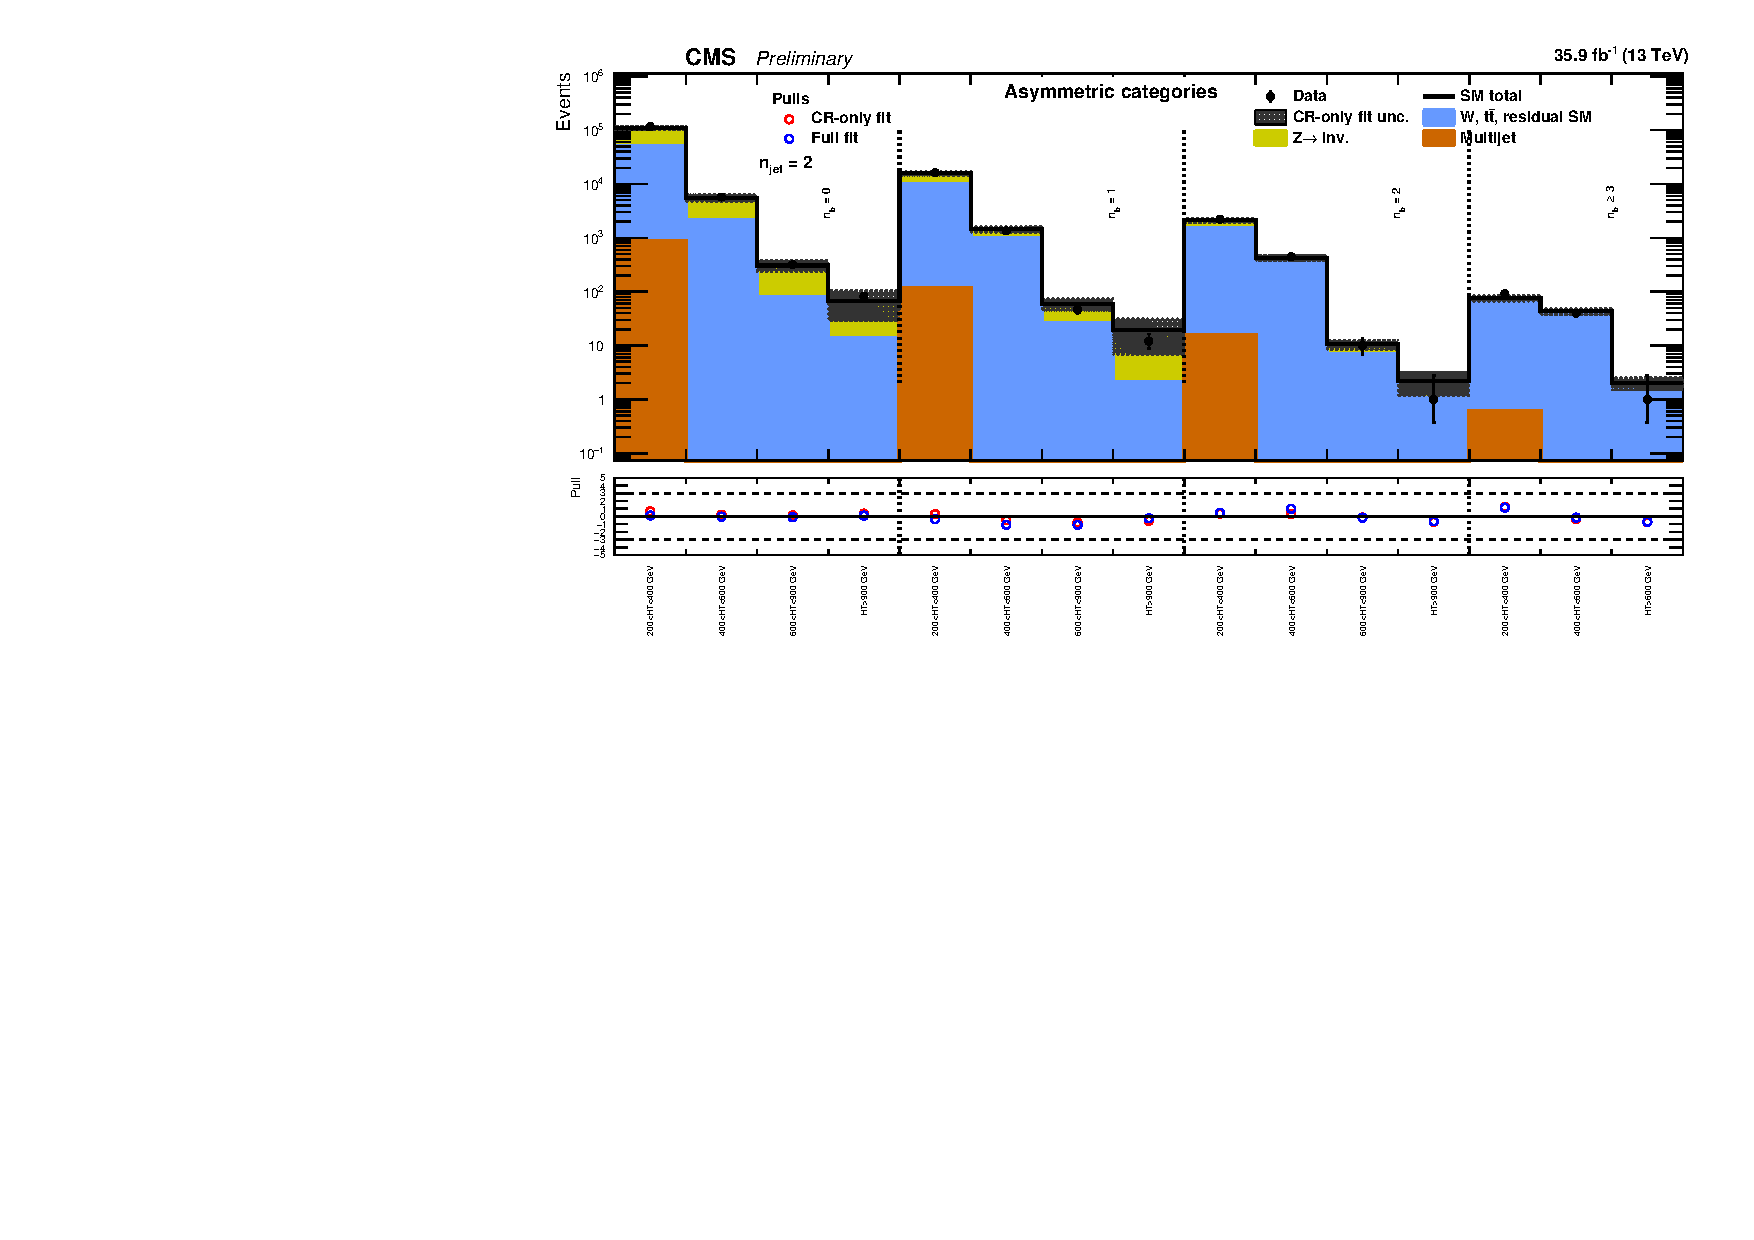
\includegraphics[width=1.\linewidth]{figures/results/36invfb_preapproval/asym/summaryPlot_Asymmetric_prefit_overlay_fit_b}
%\end{figure}
%
%% symm
%\clearpage
%\subsection{Symmetric topology}
%
%\begin{figure}[h!]
%  \centering
%  \caption{Upper panel. Event yields observed in data (solid circles)
%    and SM expectations with their associated uncertainties (black
%    histogram with shaded band) as a function of \nb and \scalht,
%    integrated over \mht, and for the symmmetric \njet category
%    in the signal region. Lower panel. Data-to-background ratios. The
%    background estimates and ratios are from the masked fit. }
%  \label{fig:mr_symm_pre}
%  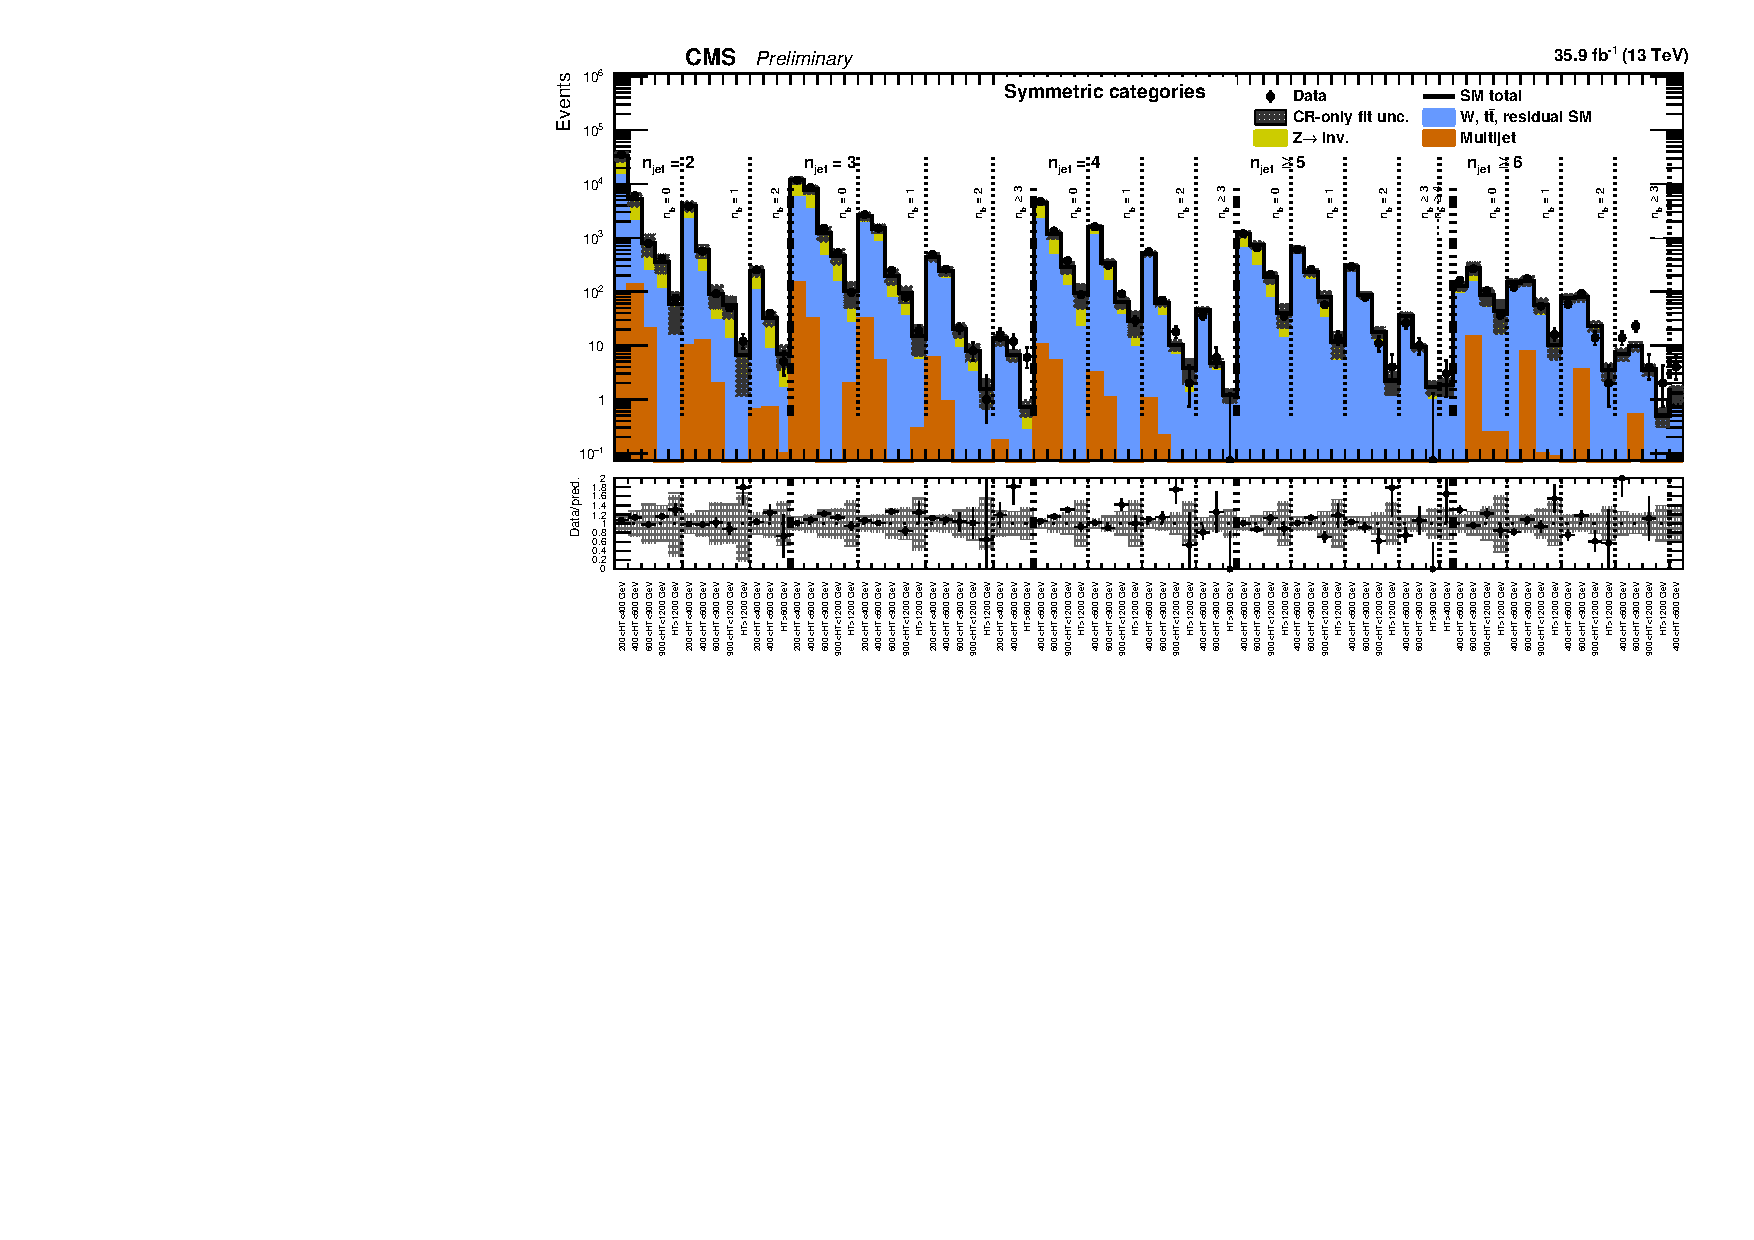
\includegraphics[width=1.\linewidth]{figures/results/36invfb_preapproval/symm/summaryPlot_Symmetric_prefit}
%\end{figure}
%
%\clearpage
%\begin{figure}[h!]
%  \centering
%  \caption{Upper panel. Event yields observed in data (solid circles)
%    and SM expectations with their associated uncertainties (black
%    histogram with shaded band) as a function of \nb and \scalht,
%    integrated over \mht, and for the symmmetric \njet category
%    in the signal region. Lower panel. Data-to-background ratios. The
%    background estimates and ratios are obtained with the full fit. }
%  \label{fig:mr_symm_post}
%  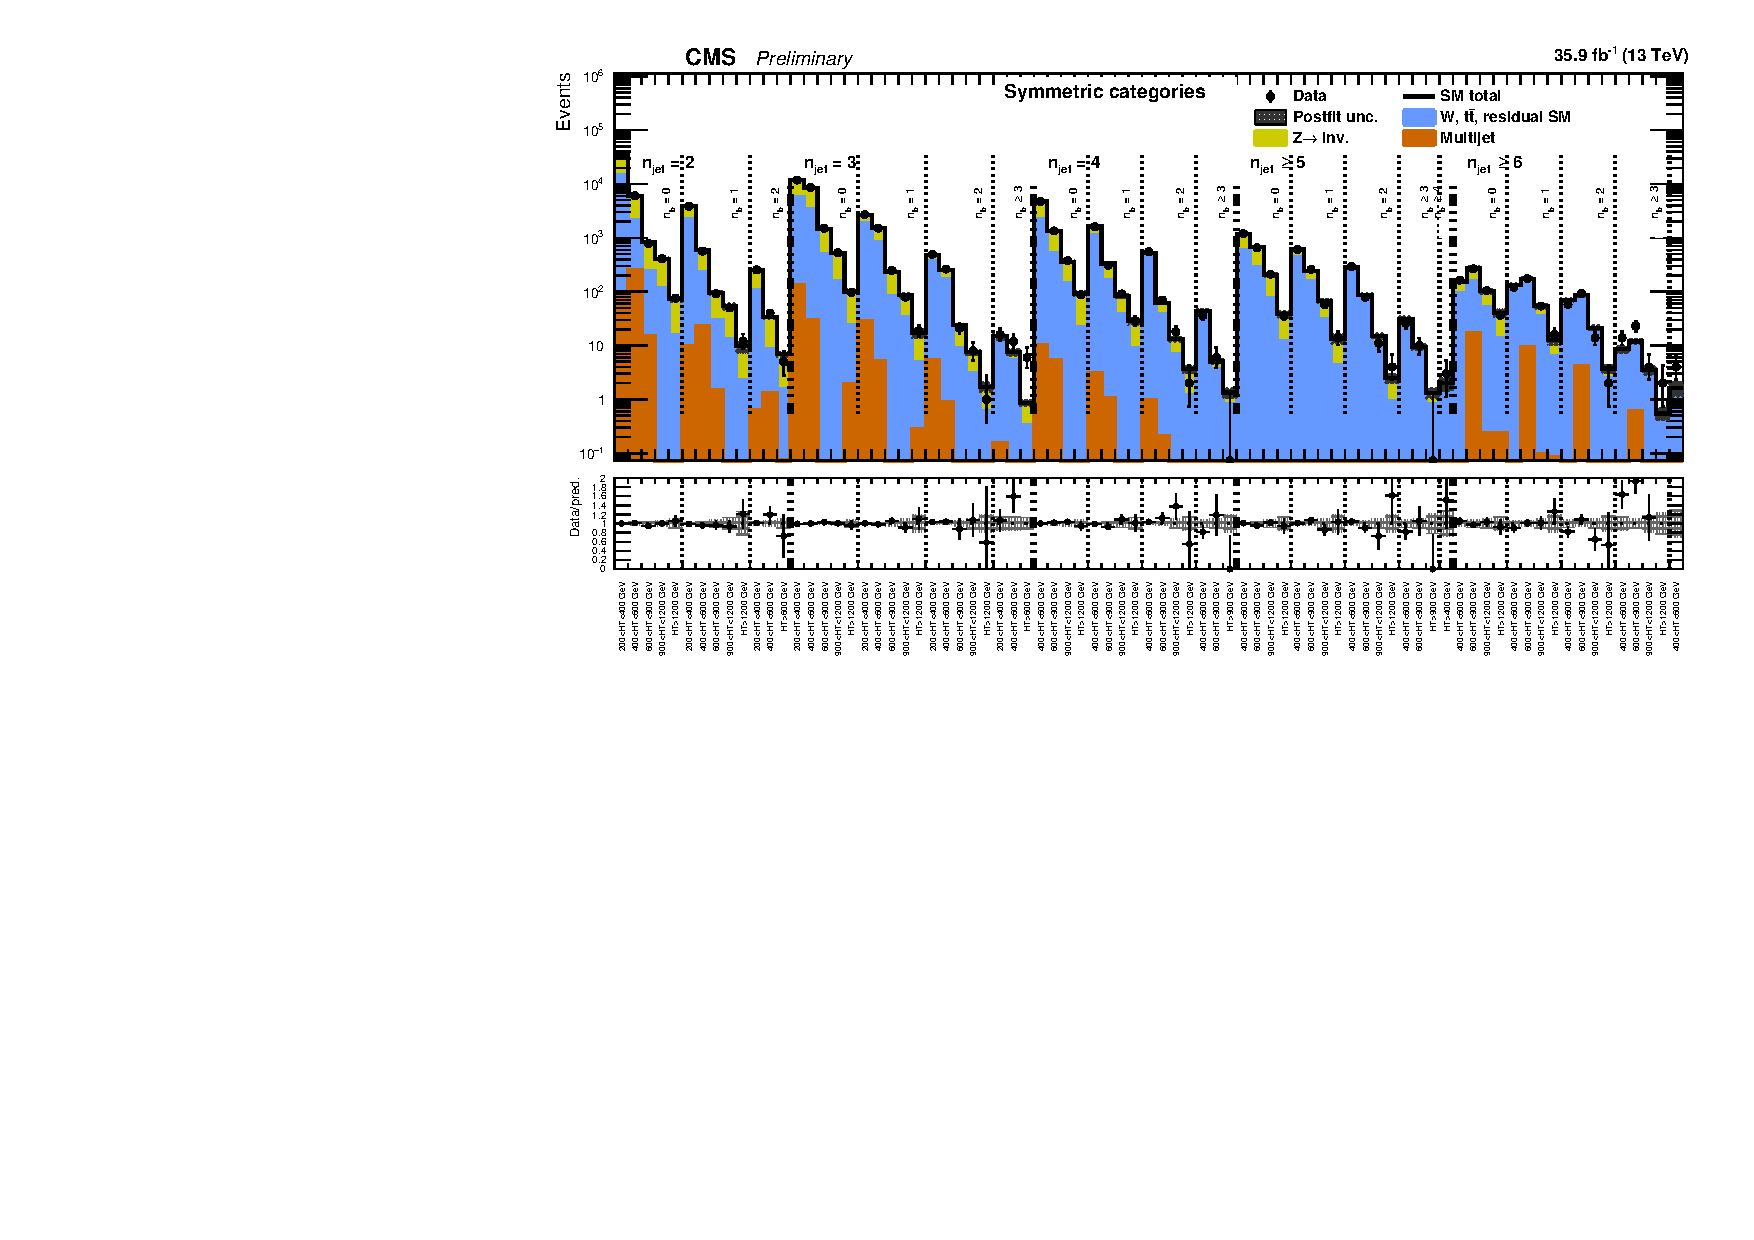
\includegraphics[width=1.\linewidth]{figures/results/36invfb_preapproval/symm/summaryPlot_Symmetric_fit_b}
%\end{figure}
%
%\clearpage
%\begin{figure}[h!]
%  \centering
%  \caption{Upper panel. Event yields observed in data (solid circles)
%    and SM expectations with their associated uncertainties (black
%    histogram with shaded band) as a function of \nb and \scalht,
%    integrated over \mht, and for the symmmetric \njet category
%    in the signal region. Lower panel. The pulls, which are obtained
%    from both the masked (red markers) and full (blue markers) fits. }
%  \label{fig:mr_symm_pulls}
%  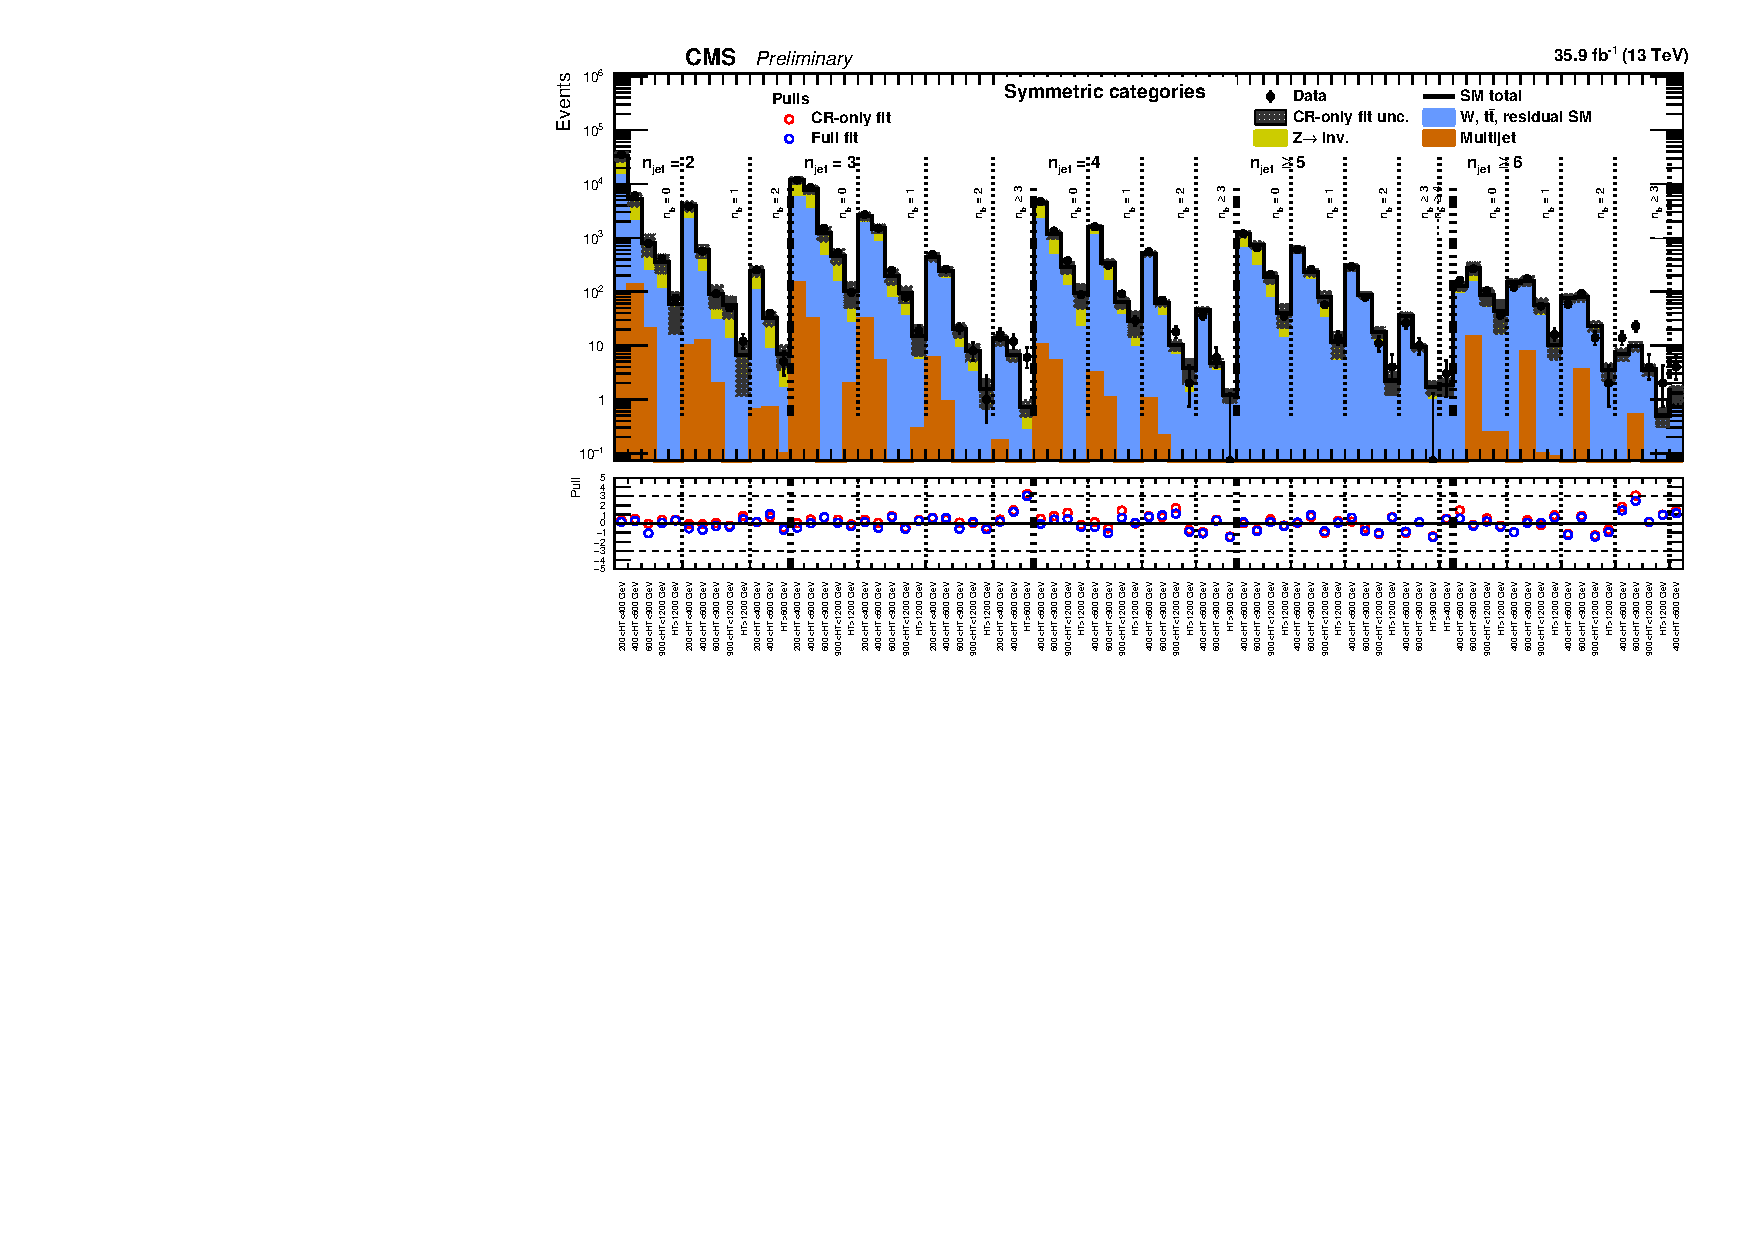
\includegraphics[width=1.\linewidth]{figures/results/36invfb_preapproval/symm/summaryPlot_Symmetric_prefit_overlay_fit_b}
%\end{figure}

% 1d histograms 
\clearpage
\subsection{Ratios and pulls}

\begin{figure}[h!]
  \centering
  \caption{(Left) Data-to-background ratios for all event categories,
    with counts integrated over \mht, obtained from the masked
    fit. (Right) Pulls for all event categories, with counts
    integrated over \mht, obtained from the masked fit.}
  \label{fig:ratios_and_pulls}
  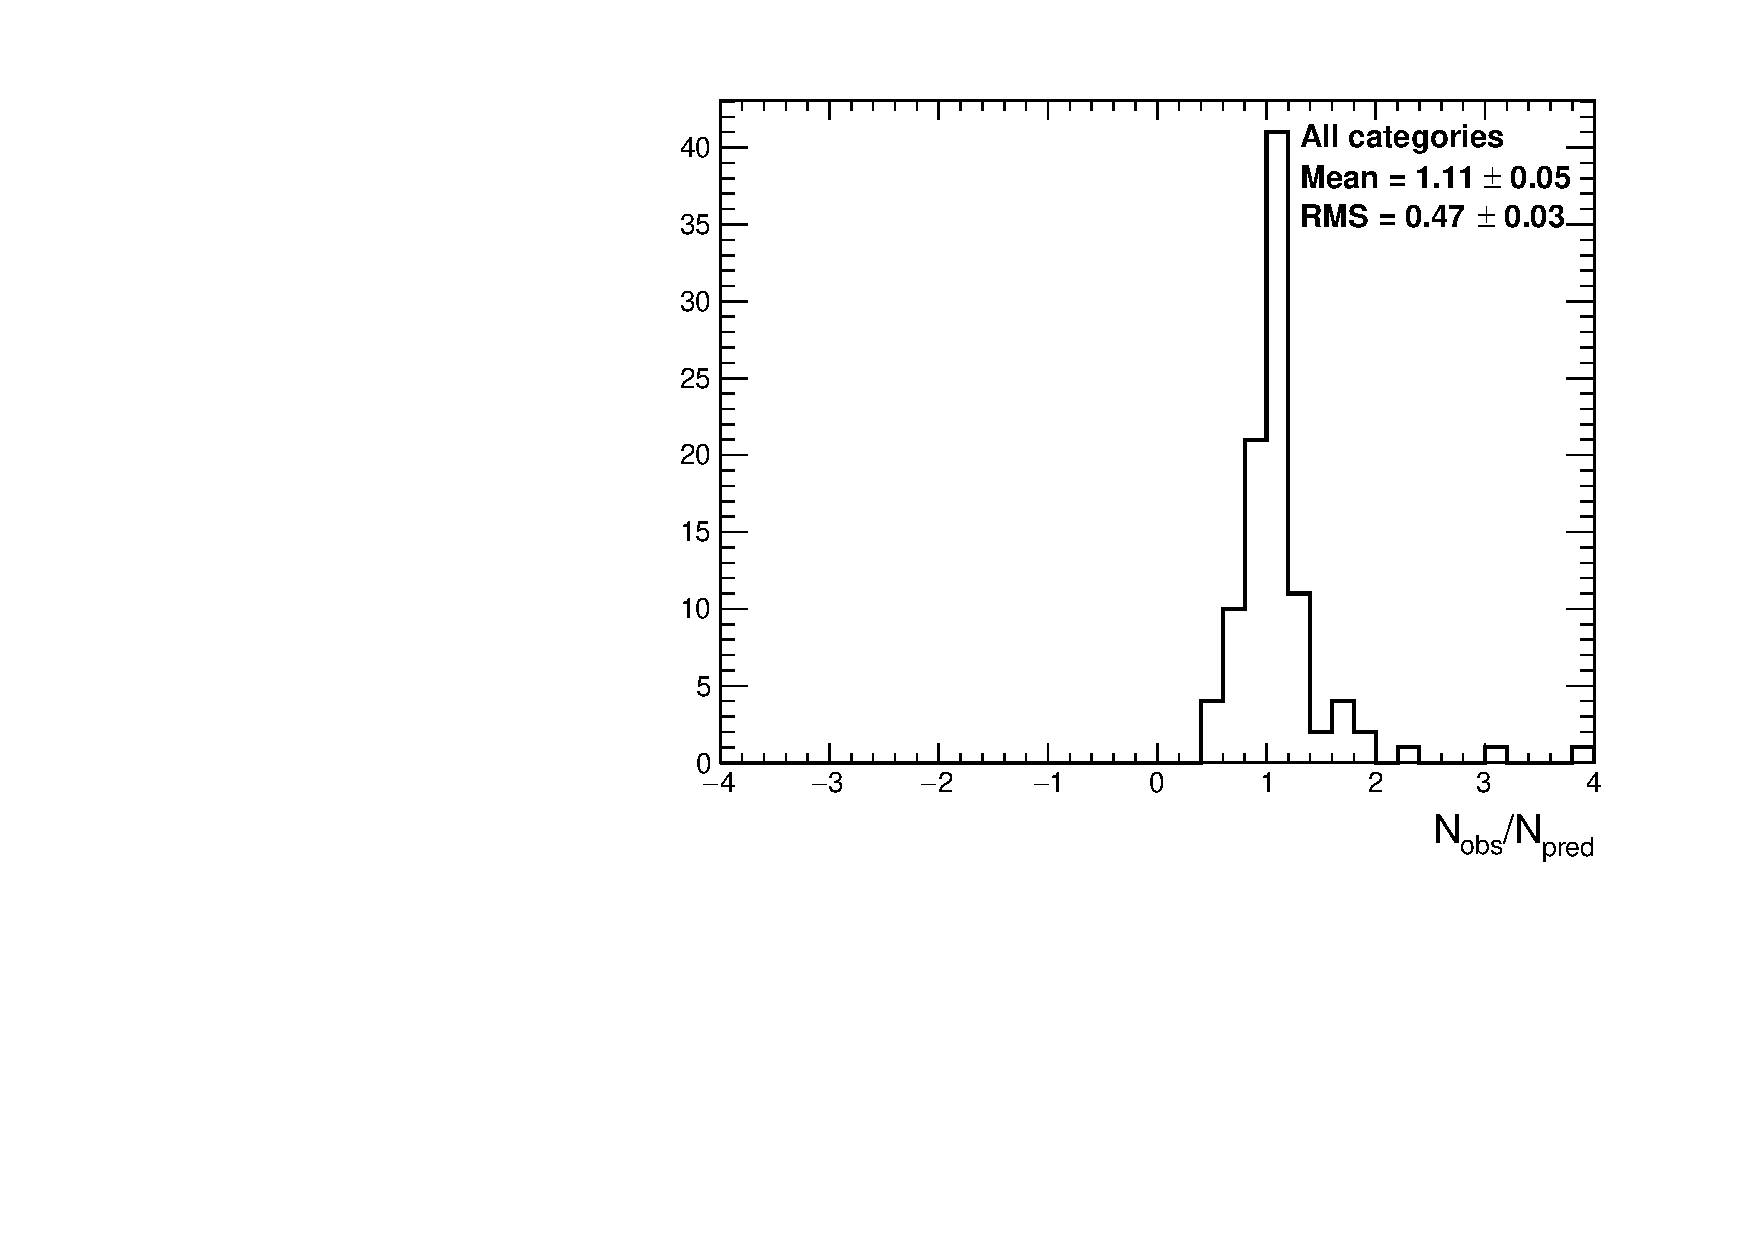
\includegraphics[width=0.49\linewidth]{figures/results/36invfb_preapproval/all/ratios_all_prefit.pdf}
  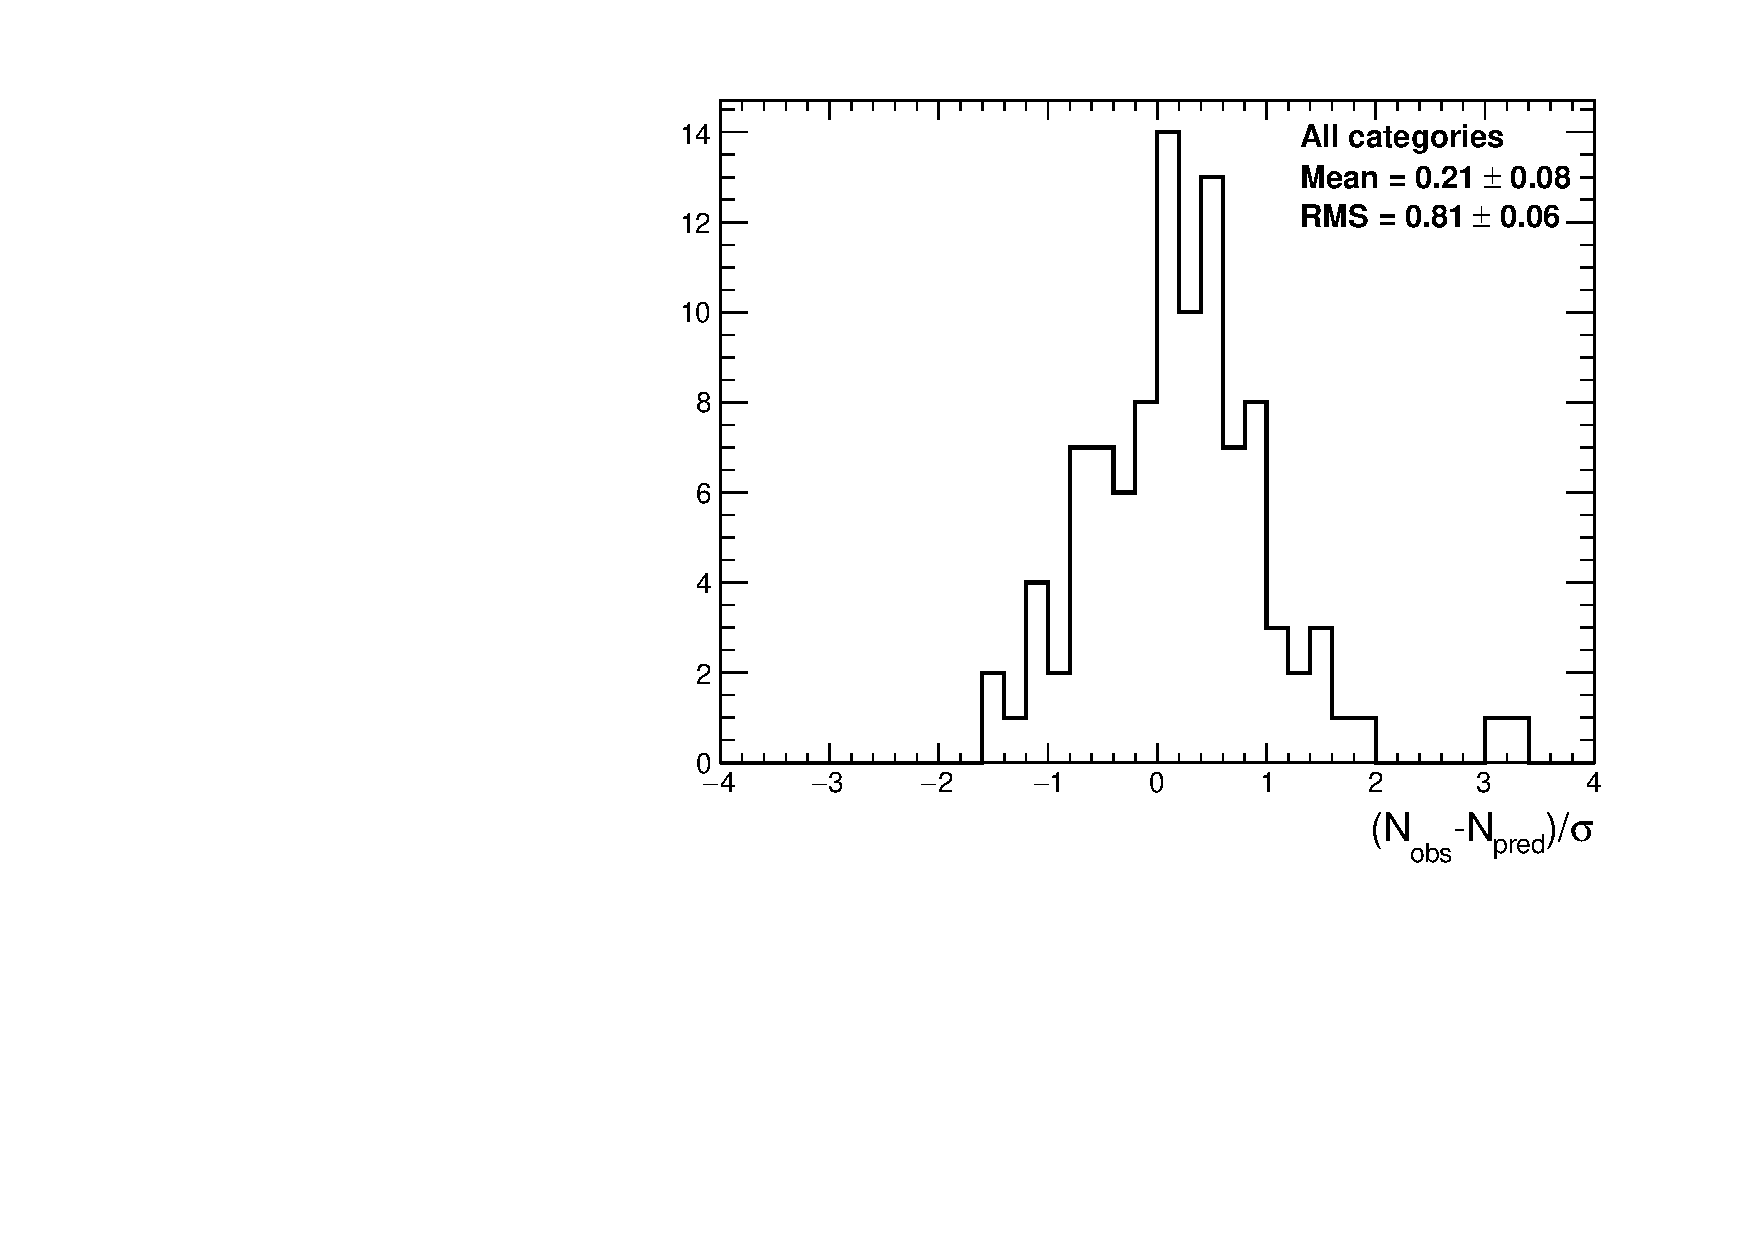
\includegraphics[width=0.49\linewidth]{figures/results/36invfb_preapproval/all/pulls_all_prefit.pdf}
\end{figure}

\begin{figure}[h!]
  \centering
  \caption{Pulls as a function of (\njet, \nb) event category and
    \scalht [GeV], with counts integrated over \mht, obtained from the
    masked fit.}
  \label{fig:pulls}
  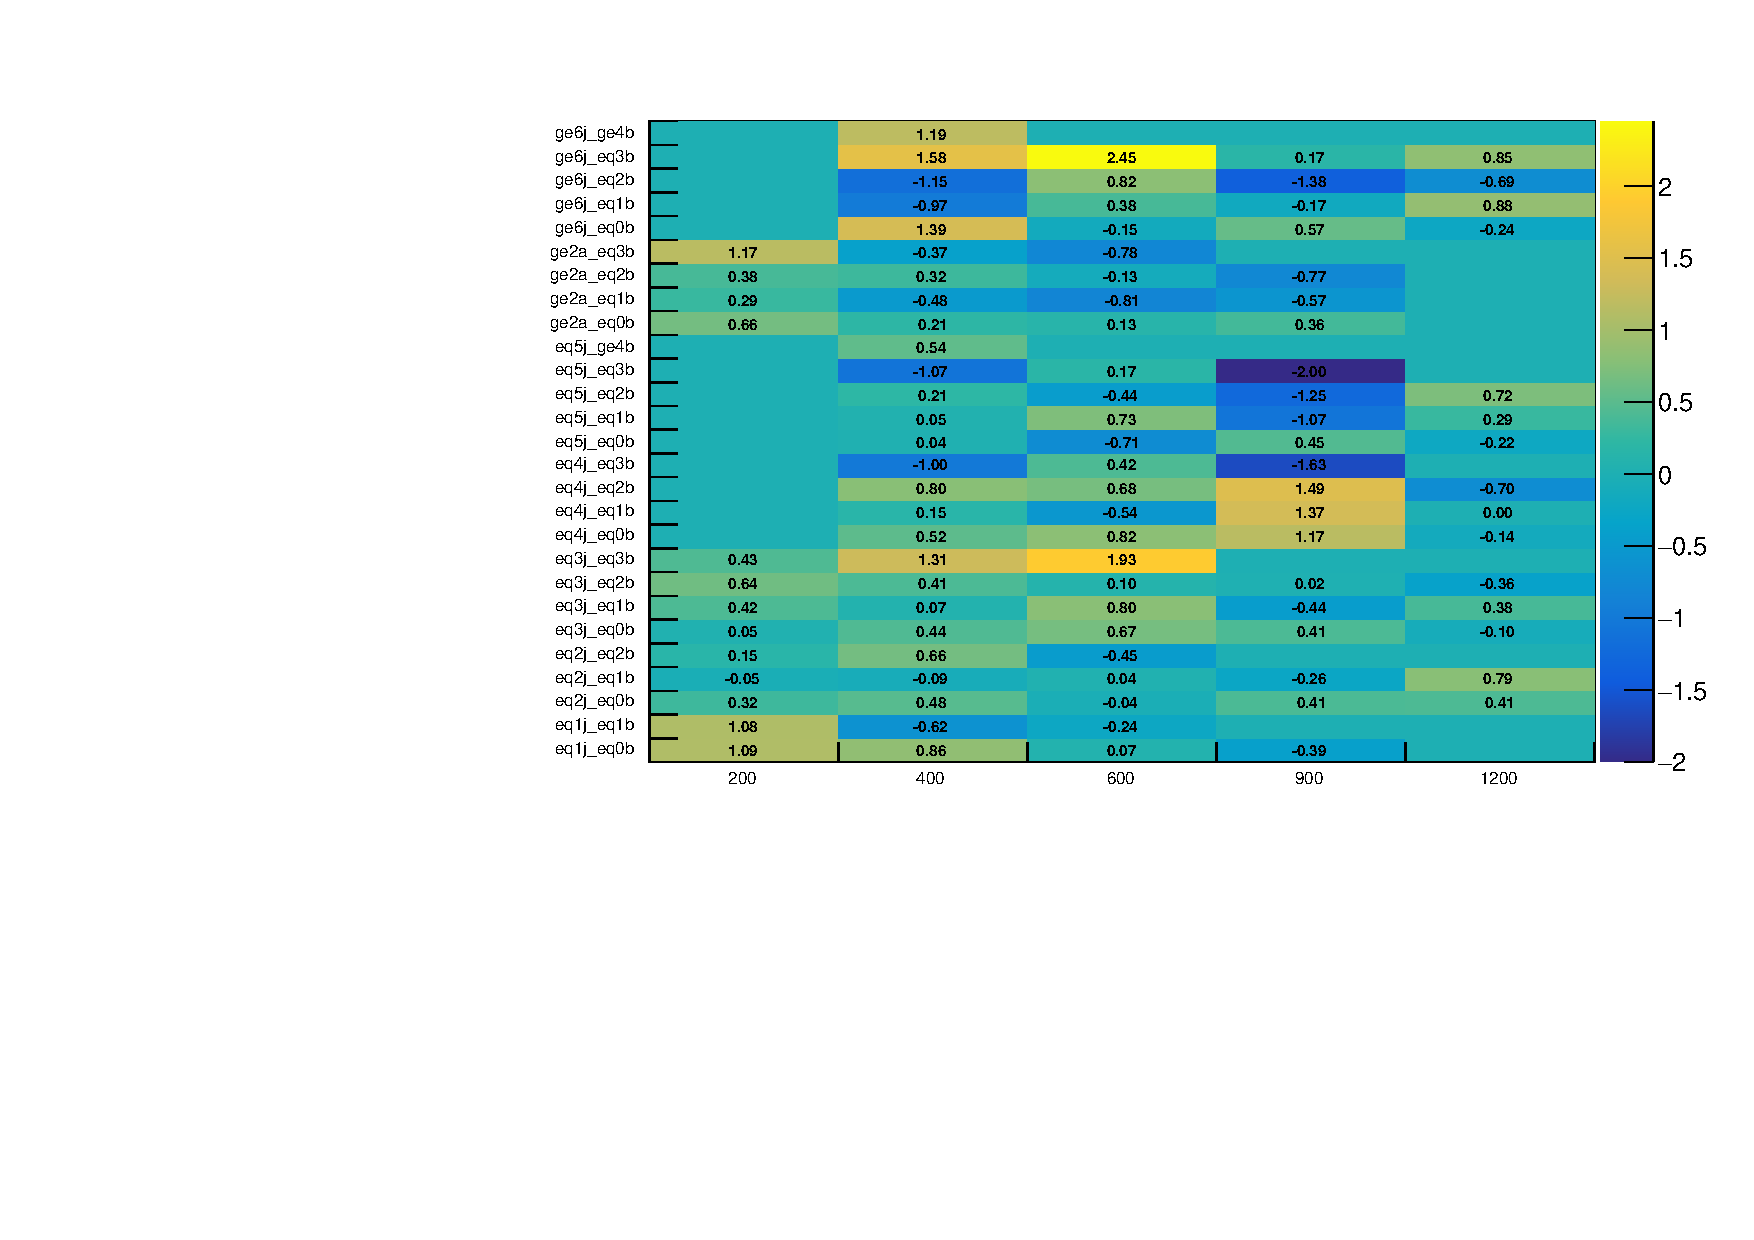
\includegraphics[width=0.8\linewidth]{figures/results/36invfb_preapproval/all/pull2D_CROnlyFit.pdf}
\end{figure}

\clearpage
\subsection{SM breakdown}

\begin{figure}[h!]
  \centering
  \caption{Breakdown of SM backgrounds in the signal region as
    determined by the CR-only (top) and full (bottom) fits.}
  \label{fig:breakdown}
  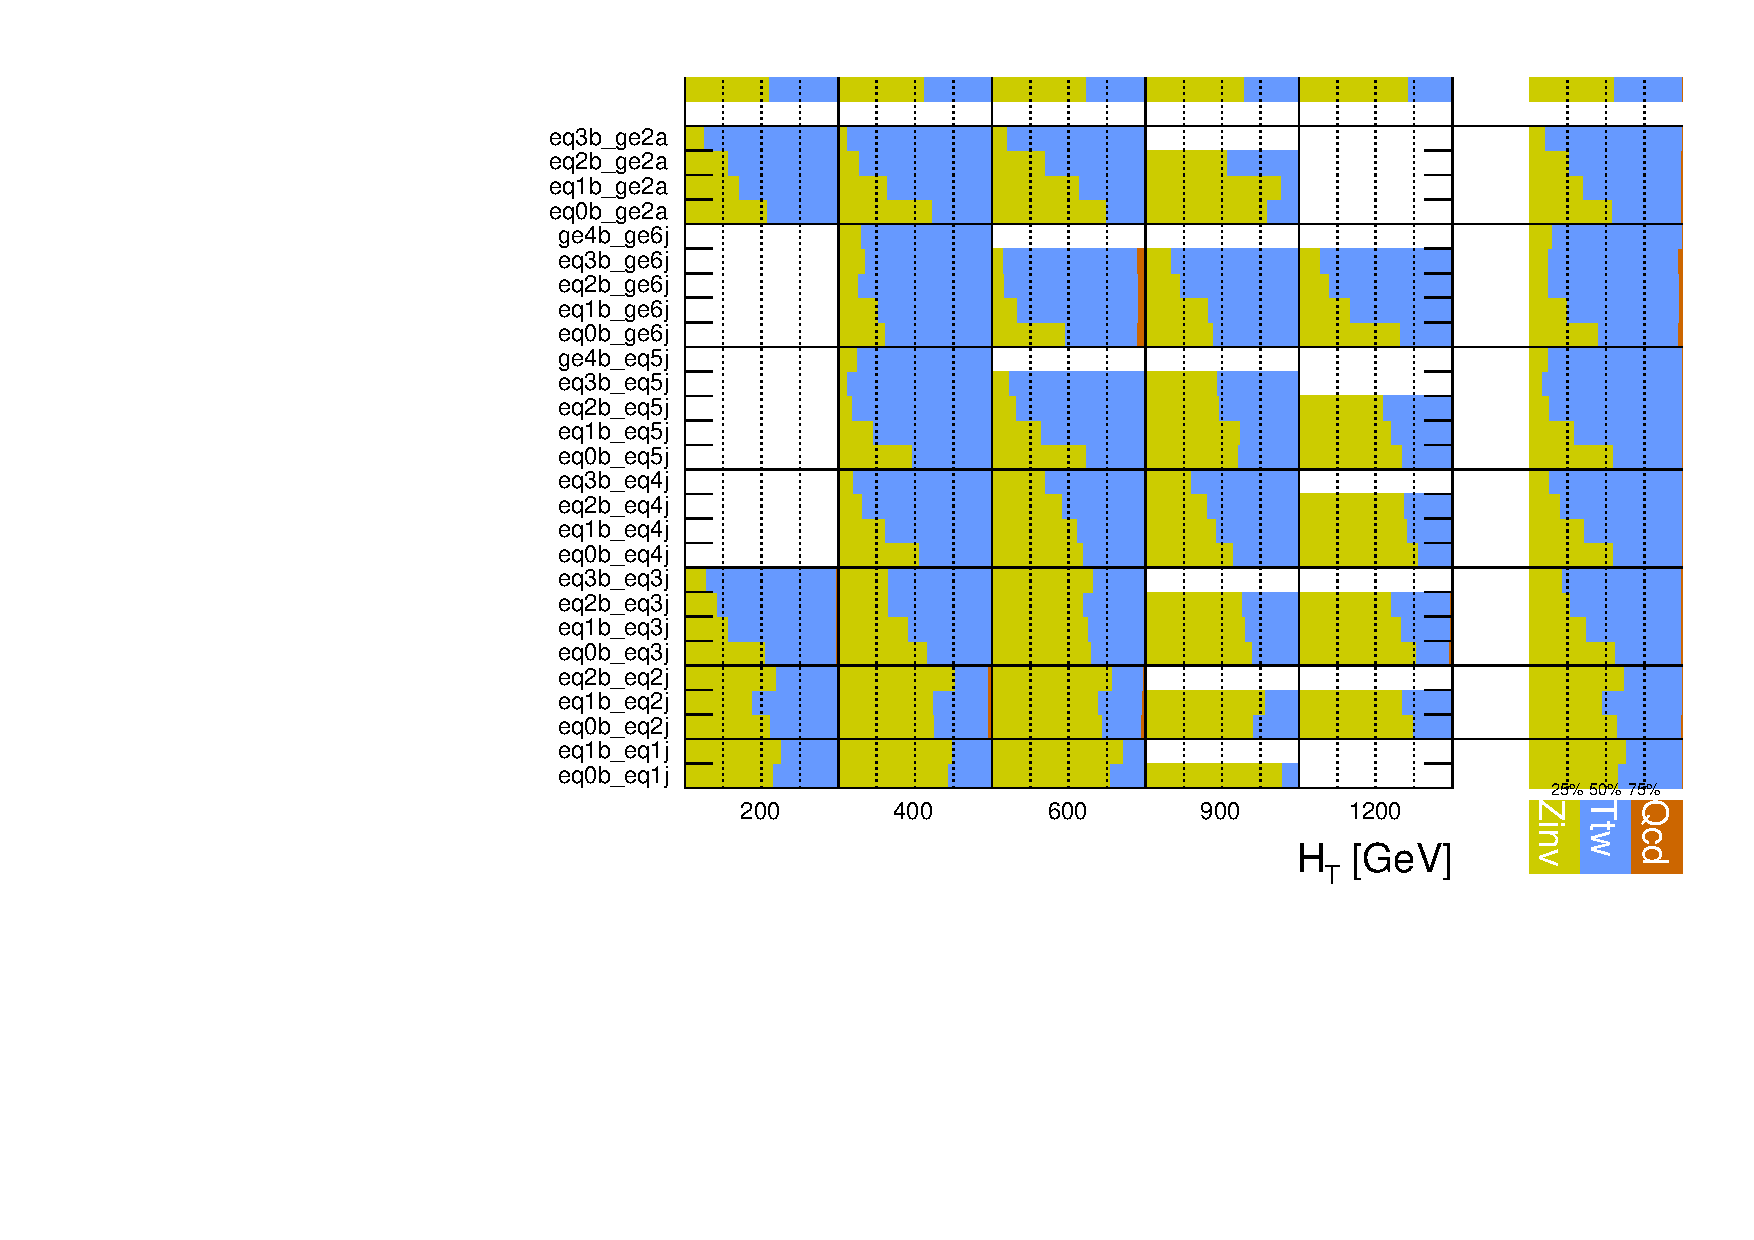
\includegraphics[width=0.8\linewidth]{figures/results/36invfb/breakdown/crfit/Signal_sample_composition.pdf}\\
  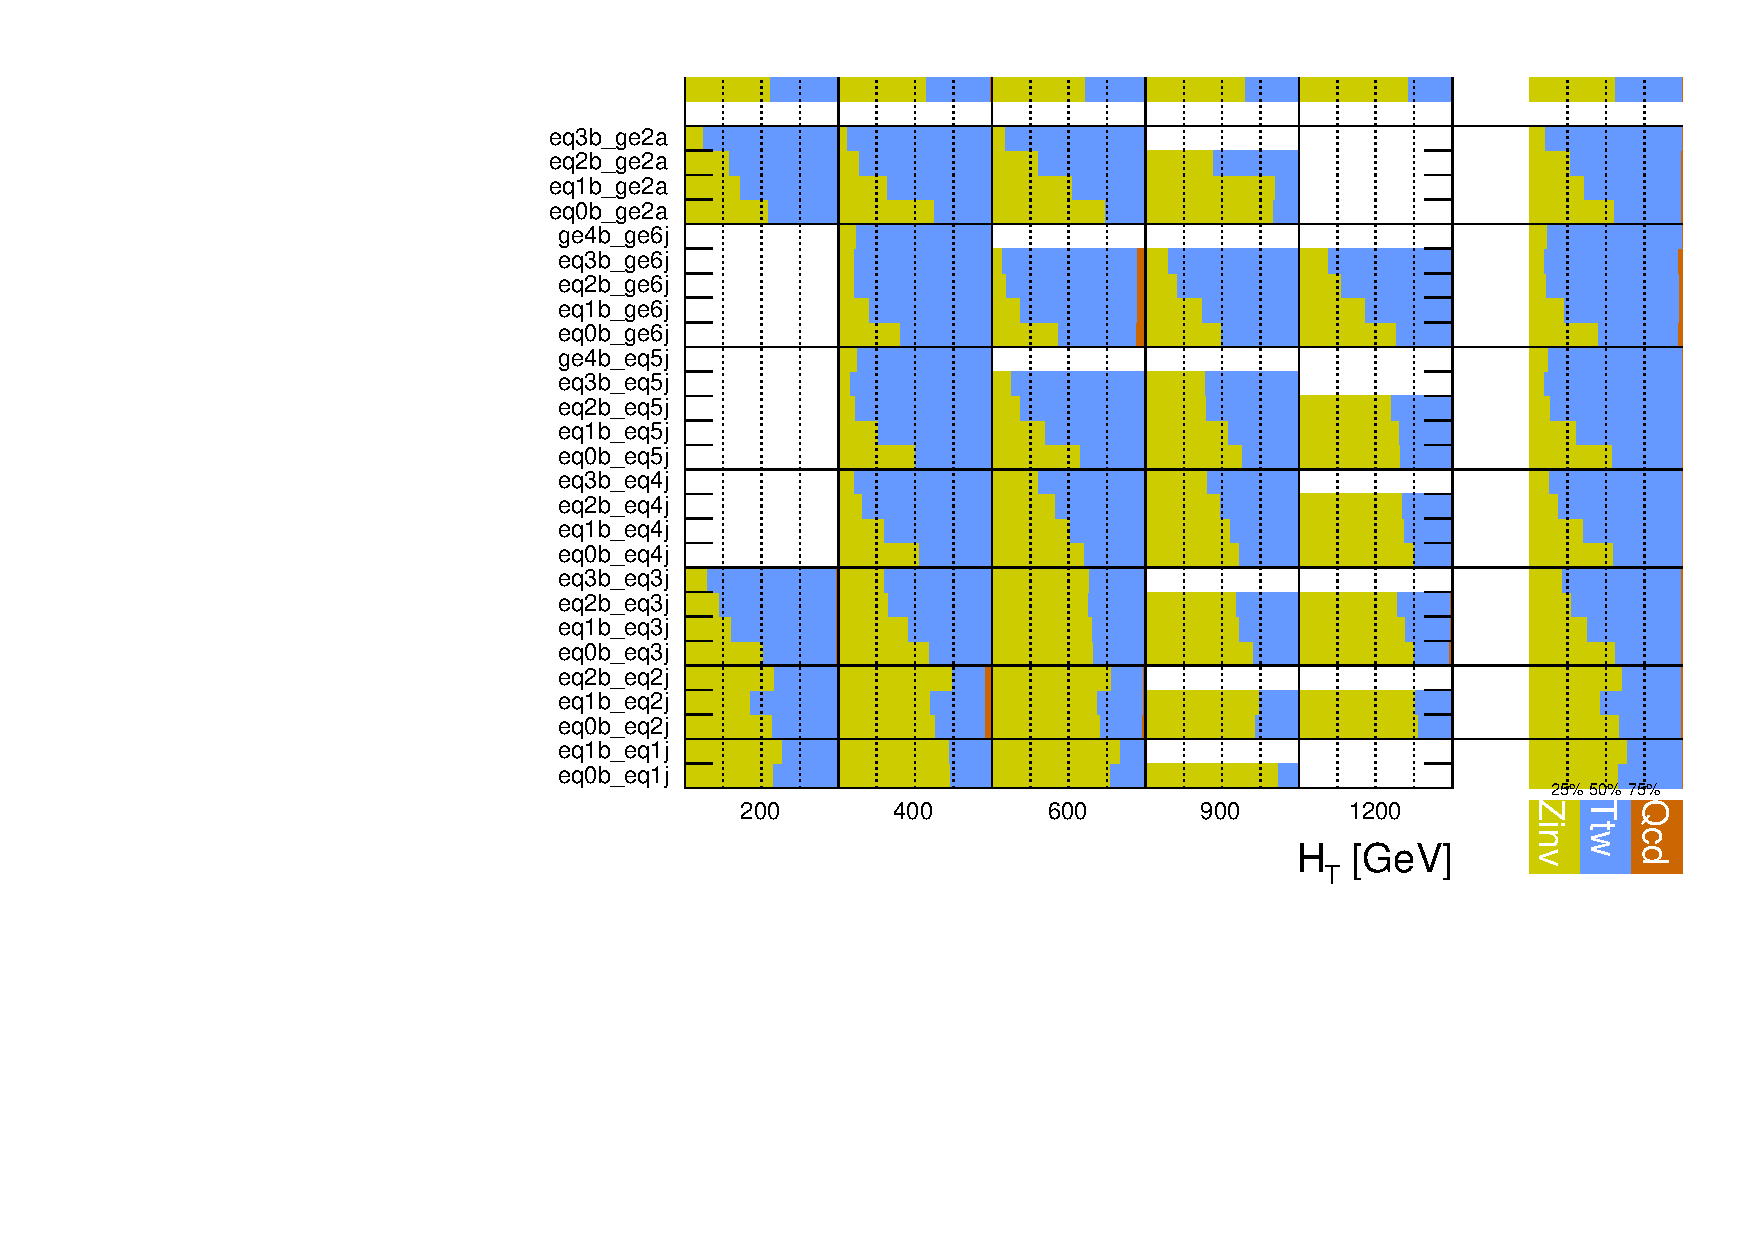
\includegraphics[width=0.8\linewidth]{figures/results/36invfb/breakdown/postfit/Signal_sample_composition.pdf}
\end{figure}

